\documentclass[11pt]{article}


\usepackage{graphicx}
\usepackage[hidelinks]{hyperref}


\title{Seminars notes}
\author{Matteo Salvino}
\date{}

\begin{document}
\maketitle
\pagebreak

\tableofcontents
\pagebreak

\section{Psychology}
These series of seminars is about the relation between humans and technology. This is a complex field of study integrating several traditional disciplines dealing either with humans such as Psychology and Anthropology or with technology such as Engineering and Computer Science. During recent years there has been a lot of work in other to combine the previous fields, for example giving rise to a new study field called Engineering Psychology. Human computer interaction community takes in consideration users who interact with consumer products and it deals with topics including the design of usable interfaces, the effect of the technology on accidental users, the development of novel ways to interact with the technology. The human factors community takes into account the operators interacting with complex system in critical settings and many research studies in this field investigate topics including the assessment on mental workload, the effect of automation on the operator, reduction of human error, etc. Users satisfaction and usability are key issues in the case of human computer interaction, whereas performance and safety are of primary importance for the other. However, in the last $15$ years both types of interactions that we wish to investigate are changed. The technology has become more pervasive and invisible, and other hand individuals are today more tech-savvy than ever before. Therefore the distinction between users and operators is now only related to the context where the interaction with the technology takes place, but usability and safety related topics belongs rightfully to the study of the interaction with any type of technological artifact. 

\subsection{The science of behavior}
Let's start with the \textbf{reflexive behavior}. In humans the crying of a baby is elicited by any uncomfortable sensation or from hanger and crying leads to parental care. So parents starts all a series of behaviors of caring for their baby that has an effect that the baby stops crying. The evolutionary history of species provides organisms that belongs to the same species the base of responses that are elicited by specific environmental condition (in this case we are talking about phylogenetic behavior). The \textbf{fixed-actions patterns (FAPs)} are sequences of behaviors, that are stereotypical, that have a phylogenetic origin. So the member of a species is involved in a FAP if some stimuli are presented called \textbf{releasing stimuli}. For example FAPs in dogs is represented by the fact that when a dog smells the urine of a rival male dog (the sign stimulus) the dog will spontaneously lift his leg to urine mark, even when his reservoir of urine is negligible. The concept of FAPs has been also took into consideration in some variability of this type of reflexive behavior. Some authors prefers to talk about \textbf{Model Action Patterns (MAPs)} which implies some degree of flexibility rather than rigid genetic control therefore accounting for individual variation. An example of MAP in humans is yawning. One particular version of stereotypic behavior are \textbf{reaction chains}. They are different from FAPs because in this case all the sequence of behavior needs the appropriate stimulation. So reflexes invariability seems to involve maintaining health, promoting survival or furthering reproduction. We refer to eliciting or activating events with the name of \textbf{unconditioned stimulus (US)}, which is a stimulus that is not related to any learning activity, but it's a stimulus that is biologically relevant and that can elicit an \textbf{unconditioned response (UR)}, that again is not related to learning, but it's the behavior following the stimulus. When we have an US that elicit an UR then this relationship is called \textbf{reflex}. The term unconditioned is used because the reflex doesn't depend on an organism's experience (i.e. learning). There are different laws of the reflex : 
\begin{itemize}
\item \textbf{Law of threshold} : there is a point below which no response is elicited and above which a response always occurs.

\item \textbf{Law of intensity-magnitude} : as the intensity of the US increases, so does the magnitude of the elicited UR.

\item \textbf{Law of latency} : as the intensity of the US increases, the latency of the appearance of the elicited UR decreases.
\end{itemize}

\textbf{Habituation} is a phenomenon that happens when we are repeatedly exposed to the same unconditioned stimulus, leading to a decrement in UR. Habituation has some general properties like the decrease in the habituated response is large initially, but get progressively smaller as habituation continues. If the US is withheld for some time, then the habituated response recovers : a process called \textbf{spontaneous recovery}. Also when habituation is repeatedly produced, each series of stimulus presentations generates progressively more rapid habituation. Habituation derives from the phylogenetic history of the organisms. So habituation has an important role in making us able to ignore irrelevant repetitive stimuli so that we can remain responsive to sporadic stimuli, typically of greater significance. Habituation has a role in psychotherapy because it's used for creating a natural decreasing in anxiety level in the absence of anxiety-reducing behavior.

\subsubsection{Respondent conditioning}
Now, let's talk about respondent conditioning. The behavior of the organisms is certain cases depends on their environmental experience. The same stimulus or event may function as either a \textbf{conditioned stimulus (CS)} or as an US, depending on its relation to other stimuli. The one trial learning and taste aversion is the association between a particular food and illness based upon a single unpleasant experience. This means that we don't have to try again the food to be sure that it gives us some troubles. However, the food may don't have nothing to do with our illness, i.e. it's uncorrelated. For this reason we define what is called \textbf{post hoc ergo propter hoc}, which is the assumption of causality based on the sequence of events plus a powerful adaptive mechanism. For most practical purposes, the conditioning procedure should arrange close temporal proximity, pairing or contiguity of the CS and US. However, it is the contingency, predictiveness or correlation between the stimuli that is critical. Thus, the US should occur more frequently when the CS is present than when it's absent : the CS should predict or signal the US. We know that when a CS is repeatedly associated with an US, the CS is able to produce the CR. The increase in the CR when there is the presentation of a CS is called \textbf{respondent acquisition}, and it's important to stress out the familiarity with CS due to the continuous exposure to this stimulus is able to delay the respondent acquisition and it reduces its efficacy. This phenomenon is called \textbf{latent inhibition}, because inhibits the learning of the CS-US relation by pre-exposure to the CS. When there is the presentation of the CS without the US, after a while we will have a reduction of the CR. This process is called \textbf{extinction}. After a while there could be a spontaneous recovery of the CR. There are two processes that we have to mention related to respondent conditioning : the first one is the \textbf{respondent generalization} which occurs when an organism shows a CR to values of the CS that were not trained during acquisition. We have also the \textbf{generalization gradient}, when the CR becomes weaker as the CS greatly departs from the value originally established by conditioning. So generalization is an adaptive process allowing the organism to respond similarly even when the condition do not remain exactly the same in different occasions. The second one is the \textbf{discrimination} which occurs when an organism shows a CR to one value of the stimulus, but not the other values. This can be realized through a discrimination-training procedure which involves both positive (CS) and negative (CS) conditioning trials. So discrimination is another adaptive learning process allowing the organism to perform differential responses to similar stimuli. There exists several temporal relations between the CS and US such as :

\begin{itemize}
\item \textbf{Delay} : in this scenario the CS precedes the US with a little bit of delay.
\item \textbf{Simultaneous} : in this case the CS and US occurs simultaneously.
\item \textbf{Trace} : in this scenario the CS happens much before than the US (i.e. we have a large distances between the CS and US).
\item \textbf{Backward} : in this case the US precedes the CS.
\end{itemize}

The second and fourth approach is not good for creating conditioning, because the CS should always precede the US and the interval between the CS and US should be kept short for effective conditioning. Next, we have the \textbf{second-order conditioning}, which extends the range of behavioral effects produced by respondent conditioning. The \textbf{placebo effect} offers the opportunity for facilitating scientific investigation with a significant impact on medical care. Of course in the real life it's not so common to have a single stimulus that can affect and be associated to an US. Many times we have what are called \textbf{compound stimulus}, where the stimuli are composed by several stimuli. In this case when we have two different stimuli that are associated with an US, we have two different scenarios :

\begin{itemize}
\item \textbf{Overshadowing} : the most salient component of the compound stimulus come to regulate exclusively the CR.
\item \textbf{Blocking} : pre-training on one component increases the extent to which that component overshadows the other. This approach has been studied by Leon J. Kamin, which discovered that responsive conditioning is selective to the best predictors of outcomes. So, in absence of selectivity, the learning mechanism would be overloaded and inefficient. The blocking effect discovered by Kamin in $1968$ is an example of selectivity based on the redundancy of a potential CS. This redundancy arises because there already exists a reliable CS for the outcome in question. When selectivity in learning fails, the organism is flooded with a profusion of potential conditioning cues and aberrant associations will be formed. So, the neural substrates implicated in selective learning effects points to a key role for the dopamine system known to be dysfunctional in schizophrenia. Studies with human participants show that the normal blocking effect is abolished in schizophrenia.  
\end{itemize}

Now, let's talk about the \textbf{Rescorla-Wagner model of conditioning}, which is a mathematical model that takes all together the things about we have talked about today. It's based on the idea that :

\begin{enumerate}
\item Learning will occur if what happens on the trial does not match the expectation of the organism, and
\item the expectation on any given trial is based on the predictive value of all of the stimuli present.
\end{enumerate}

This means that learning is all about surprise, i.e. if something is different from what we have experienced before then there is a new learning. This relates to the following Rescorla-Wagner equation :

\begin{center}
$\Delta V = \alpha \beta (\lambda - \Sigma V)$,
\end{center}
where $\Delta V$ is the change $\Delta$ in the predictive value of a stimulus $V$, $\lambda - \Sigma V$ is the difference between what actually happens ($\lambda$, which is $1$ when the US is present, and $0$ otherwise) and what we expect ($\Sigma V$), $\alpha$ represent the salience of the CS, and $\beta$ is the learning speed for a given US. The model predicts the blocking scenario that we have discussed before. Naturally there is an iterative process for estimating the associative strength of a stimulus, which describes the relations between the CS and the magnitude of the CR. A CS acquires a limited amount of associative strength on any trial. The associative strength eventually reaches some maximum level defined as the magnitude of the UR elicited by the US.


\subsubsection{Operant behavior}
In this case what is important is the concept of consequences. They are able to determine whether a behavior will be repeated or not. When a behavior has been selected by these reinforcement consequences its frequency of emission increases. On the contrary, a behavior that is not followed by a reinforcing consequence will diminish in its frequency. This process is defined \textbf{operant conditioning}, and it's the main way how the organisms modify their behavior during their life. Now, with the term we define a behavior that operates on the environment to produce some kind of effect. The operant is defined in terms of the consequences. In order to define a behavior as an operant we need to refers to a class of responses that may vary in topography, but produce a common consequence. There is a big different between operant and respondent behavior. The main difference is that in these cases the operant behavior is emitted, i.e. this type of behavior happens without that we can observe any stimulus that precedes it. Whereas, respondent behavior is elicited, i.e. it depends on the stimulus that precedes it. If we consider something that is a behavior that we probably perform in our daily life, for example if there is a notification from an application on our phone, that type of notification is a discriminative stimulus, because it makes more likely that we will behave like take our phone and open the application. In this case, the discriminative stimulus is the signal that indicates the opportunity to emit, but we can of course open the application even without that type of stimulus. So the discriminative stimulus is not enough for describing a behavior, it's just the signal. We have said that a discriminative stimulus indicates to the organism the opportunity to perform a behavior, and that's because in the learning history of that organism that behavior has been reinforced in presence of that stimulus. So, we have the events that signal the opportunity to perform a behavior, then we have the class of operants and finally the consequences that follow the operant behavior. All these three elements we call them \textbf{contingency of reinforcement}. So, we can call these three aspects antecedent, behavior and consequence respectively. E. A. Vargas in its paper entitled "On Terms" defined that antecedent refers to events occurring prior to the response of interest. Thus it's a neutral term that locates events in time and provides a point of reference for them. The term consequence, instead, implies some kind of causal relationship between the behavior that we're performing and what happens next. So, to overcome this terminological issue Vargas introduced in such paper the idea that we could use the term postcedent, which allows the placement of events in time successive to the response in the three term contingency in the same neutral manner as the word antecedent. In \textbf{positive reinforcement} we have an increase on the effect of the behavior and the stimulus that is following the behavior is presented. However, we can also have a situation in which we have a \textbf{negative reinforcement}, so the stimulus following the behavior is removed but always we show an increase on the behavior. So, the probability of performing a behavior increases not because it has been add somethings, but something has been subtracted. So, if the presentation or removal of the stimulus following the behavior decreases the effect on the behavior we have what is called \textbf{positive} or \textbf{negative punishment} respectively. Things can be either aversive or appetititve in terms of the effect that they create on the future occasions of the behavior. An interesting aspect of this consideration is that, we know that we all prefer to perform some activities rather than others, and such activities has a higher frequency wrt the ones that we prefer less. The activities that has higher frequency could actually be used for reinforcing the activities that has a lower frequency. This principle is known as the \textbf{Premack principle}. There are most applications of this principle, such as the experiments with chickens performed by Thorndike, where a chicken was placed in a closed cage and needs to press a pedal in order to open the cage door and access to food. What he was using is the time needed by the animal for finding the correct strategy to exit from the cage and access the food. However, Skinner strongly criticized this type of measure, because latency was a measure that includes both the time needed for finding the good strategy for exiting the cage, but also the time needed for all the other attempts that should have been performed because they didn't work for the animal for getting out of the cage. So, Skinner introduced another measure called \textbf{frequency of response}, that represents how many times the behavior happens in a unit of time. For representing the variations of the behavior he used the cumulative records, where the animal will receive a reinforcement after a certain number of responses. In laboratory setting what it's used for studying the animal behavior is the so called \textbf{Skinner box}, which is a cage that is equipped with a dispenser for food, a lever, speakers and some signal lights. The experimenter interacts only for reinforcing in some circumstances a specific behavior and observing the changes in the behavior (i.e. frequency of the response). Of course because a stimulus can work as a reinforcer, the animal should need stimulus. So they usually deprive the animal of food, that will increase the value of food as a reinforcer, and will determine an increase in the frequency of behaviors that serves for obtaining food. Naturally the experiments should be designed in a specific manner, because the animal does not that pressing the lever the food will be served in the dispenser. For example, the experimented has associated an acoustic signal like a click when the lever is pressed and the food is served, and also placing the lever near the dispenser. In this way, the experimenter obtains two things : the first one is that the animal associate the click for obtaining food, and the second one is the animal orientation towards the source of the sound. So, these facts will increase the probability of the animal to notice that there is food in the dispenser. This strategy is called \textbf{magazine training}. Next, if we want to reinforce the behavior of the animal to press the lever, we can associate a click to this behavior, so that we can create a conditioned reinforcer that indicates to the animal that there is food in the dispenser. One thing that people criticized of the behavioral approach is that they said that the pattern of response that is the product of an operant condition is a stereotyped pattern (it means that if we reinforce always the same type of responses there is no variability of the solution that the organism adopt for solving the problem). The idea is that stereotypy or variability, is what we reinforce is what we get. The practice of using reinforcement for modifying the behavior has been much criticized in the past, and today there are many people that are opposed to the use of behavioral strategies for behavioral change. They often make a confusion between reinforcement and reward. The concern is that rewards are experienced as a form of control and that would affect "self-determination". An analysis on $145$ experiments showed that rewards or incentives are effective for increasing the organism performance, but it's important that they are reinforcement, i.e. they are provided contingently to the behavior that we intend to increase. 

Recover 23/03/2021 and 30/03/2021 lectures

\subsection{Behavioral design toolbox and habits}
In this section we will take the knowledge that we got from the previous sections and try to apply it to design issues. The first thing that we should start with is that human behavior is programmable (of course we need to know the code). We will focus on a particular area of behavioral design called \textbf{habits}, how they work, how our products can use behavioral design to become a daily habit for our users. We are focusing on habits because they are the hardest and most important thing to get right, and therefore sustain all the other behavioral design. Behavioral design is a framework for intentionally and systematically changing human behavior through persuasive modifications of the physical 
and digital environment. So, behavioral design are :

\begin{itemize}
\item ideas and models describing and predicting how and why people behave the way they do and what they might do next.

\item practices for changing those behaviors from small to large ones.

\item tools for modifying the environment.

\item based on observations and experiments from psychology, neuroscience and behavioral economics. 
\end{itemize}

Behavioral design is not coercion or violating people's dignity, it doesn't use threats to change behavior and doesn't restrict someone's ability to act or not. There are several contributions to this field such as 

\begin{itemize}
\item \textbf{Ubiquitous smartphones} : people carry a device richly capable of sensing and changing their behavior, constantly connected to the global computing infrastructure.

\item \textbf{Advances in computational neuroscience} : we also have a clearer understandings of how the brain interacts with behaviors and how reinforcement drives engagement.

\item \textbf{Cloud computing} : the use of massive, centralized server farms has driven down the price and complexity of computing and storage.

\item \textbf{Artificial intelligence} : freely available and open-source software, from pattern detectors, prediction engines, to video courses.
\end{itemize}

So, today an application on our phone can sense an user's behavior. Now, the questions to ask ourselves are the following : is any behavioral design ethical at all ? If yes, is this particular use of behavioral design ethical ? In general, behavioral design pattern are dark or light depending on how you use them. In particular, there exists three main ethical criteria :

\begin{itemize}
\item \textbf{Transparency} : behavioral design techniques are still effective when people are aware of their usage.

\item \textbf{Social good} : design behaviors good for the individual and community is a crucial point.

\item \textbf{User's desires} : an intervention is most ethical when it's well aligned with the kind of behavior change an user actually wants.
\end{itemize}

So, reinforcement learning increases the frequency that someone performs a behavior. It focus on how habits can be induced by carefully controlling the rewarding consequences of an action. In general, reinforcement learning predictable improves how much and how often people engage with an application or product. In the literature of behavioral design what is usually reported as an antecedent or discriminative stimulus in behavioral analysis is reported as \textbf{cue}. A cue is a prompt to perform an action. Now, let's introduce the concept of \textbf{optimal challenge}. Optimal challenge prescribes that at a given moment for a given person, there exists an optimal amount to challenge someone to perform an action. If we challenge less we may not help the person to reach it goals, while if we challenge more wee may induce fatigue and the user burn out. In other concepts that we may remember the stimulus devaluation, we know that people learn through experience that certain actions will lead to positive outcomes and that is how reinforcement works. Stimulus devaluation provides a technique for destroying a learned cue-action association by introducing delay between an action and its associated reward. The resulting experience still allows users to perform their desired actions, while destroying the habit forming nature of the experience. There exists \textbf{stopping rules} that prescribes that stopping cues can be controlled to increase or decrease certain behaviors. An important aspect is the \textbf{choice of the architecture}, which is used to guide users towards a particular desired choice. Another concept is the \textbf{ambient communication} which is often used successfully to persuade people to perform an action they need to only do once. We know that people process information differently one from another. Another important concept is the \textbf{optimal information flow}, which claim that for each person exist an optimal ordering of steps for a process and an optimal density of information. Next, we have the \textbf{soft incentives}, which works by promising a future reward for an action taken today. Next, we have the concept of \textbf{sunk cost}, which can be a particularly effective way to increase the frequency of a behavior that users are already performing. Next, we have the concept of \textbf{optimal group structure}, which refers to predictable scopes and natures of interactivity between application users. While \textbf{personalization} deals with the design of products considering different user groups, skill levels or user needs. The \textbf{cognitive load balancing} prescribes techniques for how we might best display only fragments of the whole information set. So, reinforcement is the best practice among all behavioral design interventions. A habit is a programmed response to something that happens in our environment. 

\subsubsection{The CAR model}
The \textbf{Cue-Action-Reward (CAR) model} is constituted by the cue, an action and a reward. The cue plus the action creates a habit. The cue is something that the user senses in their environment that they can learn to associate with an action. In behavior design we identify three types of cue : 

\begin{itemize}
\item \textbf{Internal cue} : it's something that people senses inside themselves.
\item \textbf{External cue} : it's anything that someone senses from their immediate surroundings that causes him to perform a habit.
\item \textbf{Synthetic cue} : it's a cue that have been intentionally constructed by a behavioral designer to cue a particular action.
\end{itemize}

However, a synthetic cue may fail for one of the following reasons : either the user doesn't understand what he's supposed to do when presented the cue, or the user doesn't have the ability to do what he's supposed to do, or the user isn't motivated to do the behavior. The action is the key behavior we want an user to perform. If the actions is too easy to perform then we have wasted the user motivation, if it's too hard then the user won't do it. There exist a model that manages such trade off, called \textbf{MAT model}. According to this model, the users perform a habit when they are \textbf{M}otivation, \textbf{A}bility and with a synthetic \textbf{T}rigger. Actions are very easy to turn into an user habit, by following these simple tips :

\begin{itemize}
\item small actions are better than large actions.
\item specific actions are better than general larger behaviors.
\item make sure the person is capable of actually doing the action.
\item pick actions that are good for people.
\end{itemize}

The reward is a delightful UX change that is shown to the user instead of the standard neutral feedback. The reward the user receives for its behavior will reinforce the cue-action pairing. 

\begin{center}
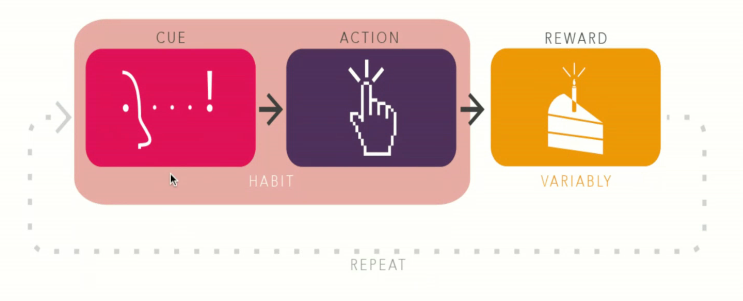
\includegraphics[scale=0.4]{./images/CAR_model.png}
\end{center}

The designers don't care about the behavior aspect, only focus on the action as the whole part of the habit. Whenever an action has an expected positive consequence specific brain regions becomes active and release the neurotransmittor dopamine into our habits system. Dopamine causes neuron-to-neuron connection to associate a particular cue with the experience of the action we are performing. The dopamine is responsible for two things : put a smile on the user face, and inducing the user to do that behavior again. The second thing is that such positive consequences have to be unpredictable, because otherwise the brain regions will not become active and in turn they will not release dopamine. The brain predictions about how good the consequence of a behavior will be, are less about what the positive consequence will be and more about when the positive consequence happens. So, carefully controlling the pattern of consequences over time is the most effective intervention that a behavioral designer can make to induce a habit.

\subsubsection{Variable reward and reinforcement}
The reward is any pleasurable positive experience that's the consequence of an action. So, reward is one of the strongest motivating tool in the behavioral design toolkit. Reward is how the brain learns what actions should be keep doing more in the future. While a positive reinforcement induces long-term behavioral change faster and more effectively than any other technique. Now, let's see the difference between \textbf{primary} and \textbf{secondary reinforcers}. Primary reinforcers have to do with fulfilling a biological need. An example of primary reinforcement would be giving a dog a treat for sitting down. Instead, secondary reinforcement occurs when a particular stimulus reinforces a certain behavior via association with a primary reinforcer. Let's say we are training our dog to sit. Every time we utter the command "sit" and he responds by sitting down, we give him a treat as a reward and tell him "good boy". We are using the food as a primary reinforcer. With time and after many repetitions, we give him less food but always follow up with the praise. Occasionally we may even skip the treat and leave the praise, and the dog will still respond to the command. The praise "good boy" in this case became a secondary reinforcer. Secondary reinforcement is more powerful than primary reinforcement because it's not tied to biological needs. Next, we need to distinguish between different types of reward :

\begin{itemize}
\item \textbf{Reward of the self} : it satisfy our desire for self mastery and proficiency. It's related to reach a complete satisfaction of ourselves, pushing ourselves to finish a project, etc. 
\item \textbf{Reward of the hunt} : it satisfy our desire for conquest. Behavioral designers often used this type of reward in games for example for setting competitions.

\item \textbf{Reward of the tribe} : it satisfy our desire for belonging.
\end{itemize}

However we have some false beliefs about rewards such as :

\begin{enumerate}
\item Rewards are for more than games.
\item Rewards are not incentives.
\item More rewards are not better rewards.
\end{enumerate}

\subsubsection{The business of habits}
Our life is defined by habits. Habits are defined as automatic behaviors that we have learned over time from experience. Social media has successfully programmed an autopilot response for the masses. So, there are four main indicators called \textbf{Keep Performance Indicators (KPI)} that are useful for potential customers :

\begin{itemize}
\item \textbf{Engagement and lifetime value} : the lifetime value (LTV) of an user is measured as their cumulative value to our product during their time using our product. So, the LTV is critical to a critical KPI to measure if our product generates revenue to usage and retention. High LTV not only guarantee us financial stability, but it also allows us to invest more into user acquisition.

\item \textbf{Referrals and virality} : when our app employs behavioral design to induce habits, our users will do more than just return more often : they will evangelize our product. Tracking referrals as a KPI will give us a greater insight into how our behavioral design efforts are driven through on motive per user and between user basis.

\item \textbf{Loyalty and retention} : to engineer a new habit is to predictively design our future loyalty and retention. 

\item \textbf{Conversions} : forming a habit quickly determines whether or not users continue use past a free trial period.
\end{itemize}

\subsubsection{Getting our team ready for behavioral design}
Let's see what we should do for getting our team ready for behavioral design. Here we report some suggestions :

\begin{itemize}
\item \textbf{Level 1: The basics} : before our team can start using behavioral design to its fullest they need to understand and value experimentations and product iterations. In this level we will discuss about four milestones our team can reach and solutions for achieving each :
\begin{itemize}
\item \textbf{Product comes first} : the product itself should be its own priority and our team should reflect that.

\item \textbf{Identify where the CAR model fits in our app} : identify the actions inside our application that lend themselves well towards becoming a habit is fundamental. Knowing what repeatable sequenced actions creates value for both us and our users will set our design process.

\item \textbf{Track engagement metrics} : it's obvious to track how are users are using our application. Indeed monitor user engagement statistics can be used to guide better product decisions.

\item \textbf{Let the right metrics guide our organization} : the default measures built in most analytics software have almost the wrong things to optimize towards. With some social training we can learn to find the correct metrics to chase.
\end{itemize}

\item \textbf{Level 2 : The best practices} : in this level we will discuss the best practices for running the organization effectively. The four milestone of this levels are :
\begin{itemize}
\item \textbf{Measure how new habits are forming} : this step is time to take those behavioral statistics that we've collected until now and to act on them. This takes our data collection initiative from being descriptive, impredictive and preventitive and in turn truly changing user behavior.

\item \textbf{Cultivate a culture of experimentation} : experimentation is the fastest way our team can learn about our product and users. Developing a culture of experimentation in a work environment where people are informed, powered and rewarded for experimentation is critical for success.

\item \textbf{Push notifications are owned by product, not by marketing} : for historical reasons marketing and messaging teams often know own responsibility for product user retention. This is most common in teams that started after the advent of the web, but before the arise of mobile. Before mobile these teams uses email to re-engage lost users or market new products to retained users. When push notification came out, it's seemed like a natural feed, push notifications are just re-engagement emails but faster. The same messaging and marketing teams becomes for designing and sending push notification and the extension of user retention.

\item \textbf{Rollout experiments regularly} : often new features rollouts are run by the engineering team. When this is true the primary success criteria tend towards "did anything break ?". If nothing broke that they continue to rollout, and once the rollout is complete everyone guess to work on the next feature. A more optimal way to do this is to empower the product team with a rollout authority. The goal should just be looking to see if anything breaks, but to monitor how the key performance indicators such as engagement and retention change, is more user coarse that receive the new feature first. If the measured behavioral API aren't changing or are changing the way that suggests that are hard things than retention and retention, the team can rollback the deployment, document what happens, explore root causes and return again with a different experiment.
\end{itemize}

\item \textbf{Level 3 : The revolution} : the revolution happens when we are able to predict engagement ahead of an experimental change, when we begin optimizing our behavioral design process and when we begin behaving like behavior first.
\end{itemize}


\section{Multimedia forensics and deepfake detection}
Today we are going to talk about multimedia forensics and next about deepfake detection. The main point of this presentation is the following question : can we trust what we see ? In the sense that if we can trust images and videos. The answer to this question is definitely no, because we know that images and videos can be easily altered. This question is very important because multimedia contents have become increasingly important in everyday life. Indeed, the expressiveness of visual content makes multimedia a powerful means of communication, however, it becomes increasingly important to be able to verify the source and authenticity of this information. The impact of fake information becomes fundamental, in the context of weaponized information and information warfare, where the organic propagation of virulent misinformation is under analysis and images and videos directly inoculate messages and have a strong impact on personal opinions. Some examples of such fake information impact are insurance frauds, crime scene alterations, reputation attacks, etc. Of course there is a new threat called \textbf{deepfake} that we are going to talk about it next time, but we would like to spend two words about it. Deepfake are spread everywhere, where there are videos that are artificially intelligence generated, they resemble someone that doesn't exist or if exists that say fictional things that are not true at the moment. The point is how can we secure an image or a video ? There are different methods to do this such as inserting something in an image that can be extracted in order to understand if something is done on the image like a digital watermarking or using some encryption method, we can insert the image into a blockchain and say of course that the blockchain itself secure the image, or we can use image and video forensics, where the hypothesis at the base is that we use only the last image we have at disposal (so it's like a crime scene). In particular, image and video forensics is about to assess origin and originality of an image or video, because it's not only the originality (saying an image whether it's authentic or not), but also is about the origin (understand the source of an image, e.g. we would like to know if an image is acquired from a certain smartphone or camera). All these techniques gather information on the history of images and videos content. Of course it's not possible to reconstruct such history in an ideal way, but is possible to do something because each manipulation to an image or video leaves on the media peculiar traces that can be exploited in order to make an assessment on the content itself. This fingerprint can be found at the signal level (the level of matrices of pixels of the image) and at the metadata/file container level. The basic principle of image and video forensics techniques, is that we have at disposal only the image, we don't have the device in our hand and we don't use external information like metadata, because they can be erased or modified. The methods we are talking about are \textbf{blind} because we don't need the reference of the original image and all these methods are \textbf{passive}, which means that we don't have to hide any mark in the picture like active methods do with a digital watermarking. So, at the end the problem is about to find some fingerprint related to some post-processing operation performed on the image, which leads to two tasks : \textbf{fingerprint extraction} (in order to know something about the image source) and \textbf{fingerprint classification} (classify the fingerprint and identify whether there are some inconsistencies in this fingerprint in order to understand if there are some manipulation on the image). So, multimedia forensics is about to assess \textbf{authenticity} using \textbf{forgery detection}, i.e. deciding on the integrity of the media and \textbf{deepfake detection}, of course \textbf{origin} using \textbf{source identification}, i.e. link multimedia content to a particular device or social network,
and \textbf{security}, in order to study if these methods built for assessing the authenticity and the origin can be studied from an adversary point of view (this is why we call this point also adversarial/counter forensics). 

\subsection{Source identification}
Source identification means different things; it's about identifying the class of devices, i.e. we have an image and we would like to say "ok, this image is belonging to for example to the class of digital camera, or to the class of smartphone". Another things that we can say about an image is if it's acquired to a certain brand or model of digital camera. Another distinction that we can do on an image is by knowing the specific device that acquired that image. If we look to the acquisition process of an image in details, if we want to known about the brand/model identification we can use for example the characteristics of the lenses, the optical filter and the CFA pattern, etc. Instead if we want to know about the device that acquired a certain image we can use information related to the imaging sensor (CCD or CMOS sensor). For example in case of a CCD sensor, we can use the so called \textbf{Photo Response Non Uniformity Noise (PRNU)}, which is caused by the different sensitivity of the sensors to light. It's a good fingerprint because it does not depend on temperature and time. Thus if we capture this noise pattern, we can create a distinctive link between a camera and its photos. So, this means that the CCD sensor, every time that we shoot an picture with our camera, impose in the image a certain noise (of course it's not visible in our image, but is the same in every image that a certain camera shoot). The PRNU fingerprint model is defined in the following way :

\begin{center}
$I^{'} = I + IK + \theta$,
\end{center}
where $I^{'}$ is the acquired image, $I$ is the image without noise, $K$ is the PRNU fingerprint and $\theta$ are other noise terms such as shot, readout, etc. The important thing that we have to notice here is that PRNU is a multiplicative noise, and it's possible to estimate with the following formula 

\begin{center}
$\hat{K} = \frac{\sum_{i = 1}^{N} W_{i} I_{i}^{'}}{\sum_{i = 1}^{N} (I_{i}^{'})^{2}}$,
\end{center}

where we simply estimate the noise of the image by subtracting from the acquired image the filter image ($W_{i} = I^{'} - I_{F}$, and then the only thing to do is to average this noise with the content of all the image. Using this formula we need to use just $20$ images to estimate a good fingerprint. Now, how can we do the detection ? Given an image $Y$, the point is to say that such image is belonging to a certain camera $C$ or another one. So, we need to estimate the presence of this fingerprint in $Y$, by means of a correlation detector

\begin{center}
$\rho corr(W_{Y}, \hat{K}Y)$,
\end{center}

where $W_{Y}$ is the noise residual of image $Y$ and the $\hat{K}$ is the reference fingerprint. Of course this correlation value is high when the image $Y$ belongs to the fingerprint, otherwise the correlation value will be low. Of course we need to set a threshold to distinguish if an image is belonging to a certain camera or not. In general, source identification is the process to link a multimedia content to a particular device. Lately source identification also deals to establish the social network of origin (also called platform provenance). We switch a little bit the problem, because now images and videos are uploaded on social networks, and so it's also important to understand if an image is original (in the sense that is not uploaded in any social network), but also we would like to understand if it's uploaded in which social network. This is important because in a forensic scenario (e.g. an investigation) it could be strategic understanding the flow that an image performed in all these social networks. We can do this by resorting at some specific traces left by each social network on the image. Of course the thing on which these techniques are based is that social networks alters images, e.g. the image is resized, it can have a new JPEG file structure, its metadata can be delete, etc. The point is that each social network do different alterations and with different rules. So, the goal of this research is to classify the images according to the social network of provenance. We would like to find these traces that are imprinted in each digital content, and in this way we would like to say to which social network each image belongs (i.e. belongs means uploaded or downloaded from the identified social network). The idea is to resort to different things; the first one is \textbf{image content-based features}, because we would like to intercept the processing that affect the image itself such as JPEG multiple compressions, resizing, filtering and so on. The other point is to resort \textbf{metadata-based features}, because we would like to take into account the changes to the characteristics of the image file such as quantization tables and image size itself. So, we propose a network called \textbf{FusionNET}, that is a CNN-based framework for addressing the social network and instant messaging application identification. We used a dual-modal features for image representation : the first one is the histogram of DCT (it's used in JPEG compression) and the other is the sensor noise residuals (it's almost the PRNU that we saw before). So, we used these feature to fed the two branches of this CNN, and then we fused together this information coming from these two stream CNN. At the end we simply classify the different social network of origin.

\begin{center}
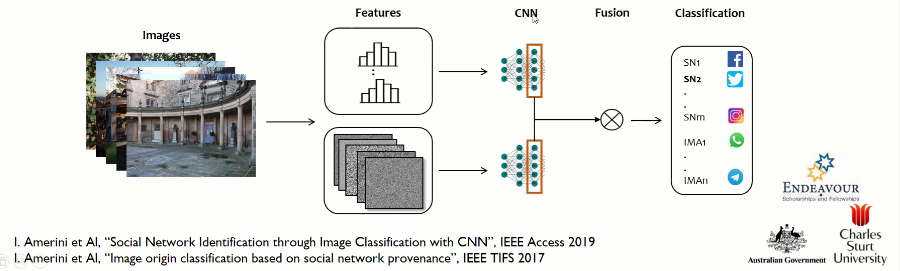
\includegraphics[scale=0.5]{./images/FusionNET.png}
\end{center}

Actually we don't classify only the social network, because we also say if an image is original, i.e. it was not uploaded on any social network. However, there is another problem, because we would like to understand whether an image is uploaded in one social network or on multiple social networks (also called \textbf{single} or \textbf{multiple shares} respectively). So that it's possible to reconstruct all the chains of uploading and downloading of an image in different social network. This problem is a little bit more difficult, indeed we tried our network but it doesn't work really well, so this is why we introduced also some features coming from metadata.

\begin{center}
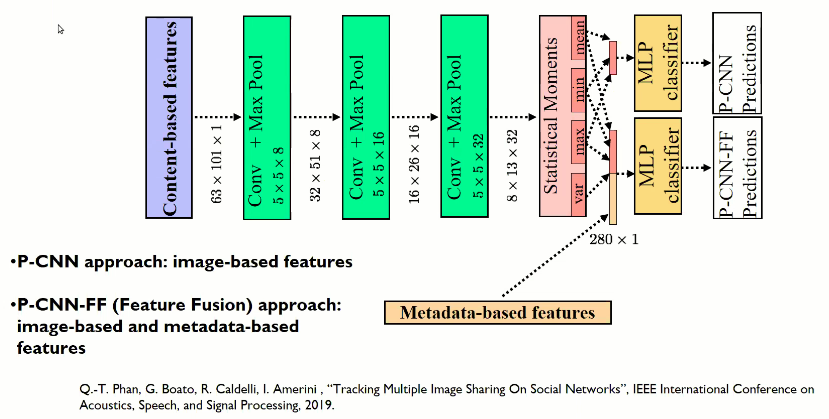
\includegraphics[scale=0.5]{./images/FusionNET_image_features_and_metadata.png}
\end{center}

We used different datasets and of course we had to build a dataset with different shares because we would like to have some control on what is done on the image, because if we download it by ourselves from Internet we don't know which transformation was applied to the image. One of the last work that we worked on is doing the same thing but from videos.

\subsection{Authenticity verification}
There are different manipulations that we are interested in forensics such as image splicing (having an image and copy a part of another image (also called donor image) in such image), copy-move manipulation (copy and paste a part of the image in the image itself) and deepfakes. So, the point is how an image that is manipulated can be revealed and localized ? We work with only single probe image, and we would like to detect if the probe was manipulated and provide one or more masks on where there is a manipulation. So, we analyze the image with different patches, we pass it through a detector with machine learning techniques, and then the output is the image with a localization map and we would like to say if this image is doctored/manipulated with a certain confidence. There exists several techniques for tampering detection and can be divided in four categories :

\begin{itemize}
\item \textbf{Camera-based} : they are related to the PRNU discussed in the previous section. We have a tampered image and if we found some inconsistencies in the PRNU estimation, then they can be a hint of the fact that the image is manipulated.

\item \textbf{Physics-based} : these techniques are based on illumination and trajectory. Illumination because it's really difficult some times to reproduce the lights of the image to reproduce its real illumination. Trajectory are mainly used to detect videos where some movements are manipulated.

\item \textbf{Format-based} : in this case we can leverage the information coming from the image compression. Of course is something is done on the image, this image needs to be double compressed. If the double compression is done only on a image region, these inconsistencies can be detected and thus it's possible to say that the image is manipulated.

\item \textbf{Features-based} : in this case we exploit some salient points in the image such as SIFT or SURF, in order to say if the image is fake or not.
\end{itemize}

A relation to the last category we want to talk about the \textbf{Copy-move forgery detector (CMFD)} method, which detect fake is applicable only on the kind of copy-move forgery. This is one important works in forensics because was the first time that was applied computer vision techniques to image forensics research problems, that since that time implied some signal processing techniques. The idea behind the copy-move technique is that when we perform a certain copy-move in the image we usually use a geometric transformation in order to take a part of the image and then copy this part in another part, but may we need to first of all translate it, and then we need to rescale it or rotate it, and doing some affine transformation in order to fit well in the part that we want to cover or duplicate. The point is to detect such copy-move and to estimate this transformation that has been performed in order to fit this part that we would like to copy in another part. The idea is to resort to the salient points. In this case we use \textbf{Scale Invariant Features Transform (SIFT)} (they are robust to the transformations that we've discussed before), which are usually adopted for their high performances and low complexity. The detector that we proposed in the first phase extract the SIFT features from the input image and match them in the image. In the second phase we cluster and there is the effective forgery detection, and then apply the geometric transformation estimation between the matched clusters and through the usage of correlation mask and segmentation we were able to localize the duplicated region. Of course this method works also on printed images, and for this reason we developed a smartphone application in order to detect this kind of fake. Now, the question is can a manipulation be revealed and localized with a CNN ? So, we would like to find an universal method able to detect all the kind of attacks. We start by using CNN in order to understand if it's able to detect double JPEG compression, because there were statistical methods based on the histograms analysis, since the histogram of the DCT coefficient changes a lot when the image is double compressed. For this reason, we can use machine learning techniques to build a detector that can distinguish between single quantized histograms and double quantized histograms, and this would be a good start in order to detect an universal method to take all the problems of forgery detector. In this work we evaluate three CNN architectures : spatial-domain (RGB patches), frequency-domain (DCT coefficients) and multi-domain CNN (a combination of the two). We don't have any assumption on tampering patches for training, differently from some state of the art. For example, the multi-domain CNN learns the intermodal relations between RGB features and histograms. At the moment we are working to a project related to car damage manipulation detection, because the insurance companies have this software in order to detect automatically damages in a car and also to link the damage with a certain money value of it, but some times these images are manipulated, and thus is crucial for these insurance companies to detect these manipulations. The point that i said to you about the universal method is not solved yet, because the independence from kind of manipulations and compressions is not solved. Furthermore, this tool for forgery detection needs to be deepfake aware. Now we are going to investigate multimodal approach in order to say something about the originality of an image, that means we would like to consider not only images and videos, but also text and understand if there is some kind of semantic inconsistencies in the all of these three media. The importance of this topic is represented by the fact that big companies like Facebook are investing tons of million of dollars in order to solve this kind of problem. Another point that needs to be addressed in the future is the multimedia forensics in the wild, i.e. all the concepts that we have talked about still holds if the image is shared on social networks ? So, in order to preserve the trustworthiness of data shared on social media, we need to address also the problem of studying images and videos in the wild. Another point that is necessary to address is a tool for verifying machine learning and deep learning models.

\subsection{Deepfake generation}
There are several definitions for deepfakes : someone will say that they are face manipulations in images/videos, someone will talk you about photoshopped images, someone will argue that they are also everything in computer graphics and of course they can also be seen as deep learning based methods that can be used to generate these fake videos (indeed the term deep comes from deep learning). According to Wikipedia deepfakes are synthetic media in which a person in an existing image or video is replaced with someone else's likeness. A general definition for deepfakes is the following : they are manipulated images and videos of faces. Usually, at least at the beginning, the term deepfake was used to refer to a kind of deepfake called \textbf{face swap}, in which we have a source actor and a target actor, and we want to move the face of the target actor over the face of the source actor. Of course we can use several techniques to do it like encoders/decoders architectures, however the face that we will obtain will not look exactly as the target actor face. So, even though this method can be of course used, today this kind of applications are not such realistic. However, there is also another way to generate deepfakes, in which we can take the source actor and we want to reenact the target actor, i.e. the source actor will say and do whatever the target actor will say. This kind of contents are much more realistic wrt the ones of the previous case, and indeed most of the times this swap has been used to generate super realistic videos until now. However, deepfakes are not just AI based techniques to generate fake videos, and in fact fake faces and movies have been produced for a lot of years right now. However, most recently some other techniques based on deep learning method have been introduced and this kind of contents can be generated through artificial neural network. They can still looks realistic and this kind of contents can be also much cheaper to produce wrt to the one produced using the previous technique (couple of seconds against hours). So, let's start from the Face2Face method, which is a reenactment method. In order to do it, first of all we generate a 3D model in such a way to minimize the distance between the input and target face. So, we construct a parametric model, where each parameter controls some characteristics of the video like the color of the scheme, and then we point to fit such model to RGB image that looks exactly the same to the one of the target actor. Next, we can start to assign it some more subtle changes like add the mouth, eyes, and we will end with a 3D rendered model that looks like a realistic person. Finally, we can transfer the expressions from the input source actor to the target actor. At the end we will put this 3D model on the target actor face, and he will look exactly like the real person, but reenacted through the expressions of the input source actor. As we seen until now, there are different ways to generate deepfakes. We've seen the difference between face swap and face reenactment and we have also a discussion about the difference between computer graphics and deep learning based methods. Of course deepfakes have a lot of applications such as in entertainment, advertising and movie production. However they are also very dangerous because they can be used as weaponized information, or for manipulating public image of celebrities and politicians, etc. Of course there has been a lot of attentions on this kind of content during the last few years. Some social networks started to ban deepfakes.

\subsubsection{Generative models}
We know what discriminative models are. We give a set of features as input to the model, we train the model on it, and the model will return a certain probability distribution over a set of classes for the input features, i.e. our goal is to learn $P(Y \mid X)$, where $X$ is the features set and $Y$ is a target class. On the other side, we can also generate new images and this is what a generative models tries to achieve. The main difference with the discriminative models is that here we provide a random noise $\zeta$ and a class $Y$ as input to the model, and we want to generate features $X$, i.e. our goal is to learn $P(X \mid Y)$. 

\paragraph{Variational Autoencoders (VAE)} We will start just with an overview of \textbf{Variational Autoencoders (VAE)}, which are one the techniques that can be used to generate deepfakes. The VAE are structured in the following way : there is the network called encoder/decoder network, where the encoder takes an input image and it maps this image to a latent space (it's like a compressed representation of the input image), and next we provide this information as input to the decoder, which learns how to reconstruct starting from the input image compressed representation the input image. Once we trained this model to achieve the aforementioned task, we can of course just take the decoder part, sample a random point from the latent space representation, and we can use the decoder to generate new realistic images. 

\paragraph{Generative Adversarial Network (GAN)}
On the other side there are the Generative Adversarial Networks (GANs), that works in the following way : there the a network called generator, which takes a random noise as input and generate fake images, and we have another network called discriminator that instead tries to discriminate between real images and fake images generated by the generator. Once we have trained these two models, we can just take the generator, feed it with a random noise and try to generate new images as well. So, we are now going to focus on this kind of networks. The way they work as the name suggests is through an adversarial game in which the generator wants to full the discriminator with fake images, and the discriminator is trained instead to catch whether an image is fake or not. So, they are trained through an adversarial objective, in which the discriminator wants always to discriminate between fake and real images, while the generator wants to full the discriminator (they play one against the other). In order to train the discriminator, at each training step we take fake and real images, we measure an output and we measure a cost function that tell us whether this prediction is correct or not. This cost function will tell us if the discriminator is working well, and if not it will help the discriminator to update its own parameters that can be updated and used in the next step to make better predictions. In our case we used the binary cross-entropy cost function, but of course there much stronger cost functions that can be used. Next, at the same training step we also want to train the generator and update its own parameters, if it's not still working well. The way we do it is by taking the output prediction, we calculate the cost function and we update the parameters of the generator. Notice that the generator will maximize the cost function, while the discriminator wants to minimize it. The best GAN to generate deepfakes was developed in $2018$, which is called \textbf{StyleGAN}.

\subsection{Deepfake detection}
The detection of deepfakes is possible, because the methods used to generate them are not perfect, and thus we can leverage some defects in order to detect them. There are a lot of datasets that we can work on deepfakes. At the moment we can leverage visual artifacts (such as color anomalies and sharp boundaries), there are semantic inconsistencies (different eyes color or ear rings) in the face that we create with that technique that we can exploit, it's possible to extract some camera-related artifacts (in this case we use PRNU based methods, because the deepfakes do not have any camera fingerprint), it's possible to detect deepfake because there are inconsistencies in the identity that we are going to generate (e.g. the expressions of the real person are not exactly recreated in the deepfake), and also because GANs themselves introduces some fingerprints in the image that is possible to extract in some manner (GANs present specific artifacts due to the peculiar generation process). Today there exists several detection strategies we can use to detect a deepfake, such as feature-based, learning-based and sequence-based methods.


\subsubsection{Feature-based methods}
\textbf{Eye blinking} is a feature-based method, because in the deepfake the eye blinking was not really shown and this is a good characteristic to exploit in order to understand if a video is a deepfake or not. The authors that introduced this technique first of all detect the eyes of the person in the image, and then feed a recurrent network in order to understand if there is eye blinking or not. Then they check how frequently this phenomenon happens in the video and at the end they could say whether the video is fake or not. Another recent work presented $2020$ is called \textbf{Heart variations}, where the goal is to check if in a video is possible to detect the heart variation. It's possible to estimate from videos the blood movement through the veins, because it changes the skin reflectment over time, and so it's possible to understand the hearth bit of a person. So, if it's possible to do that then this means that the person is real, otherwise we can simply say that the person is not real. It's possible to estimate the heart variation studying the PPG signals, and the authors of this technique constructed a neural network which takes in input such heart variation estimation in order to classify in a video is a fake or not.


\subsubsection{Learning-based methods}
The main point of these techniques is to have first of all a face tracking method, where we extract the region of the image covered by the face and then this region is fed into a learned classification network that outputs the prediction on the RGB patch. The classification is based on XceptionNet pretrained on ImageNet. The difference wrt feature-based methods is that here we fed the network with a frame of the video. In the test phase we feed the network with a frame of the video, we select the extract the face of person in the frame, and we run the classification network, which outputs a prediction that can be fake or not. The problem is that they learn to be really good on specific datasets and manipulations, but they didn't generalize so well, because they network overfits too much. Indeed, this issue is called the \textbf{generalization issue}, because state-of-the-art deepfakes detection methods are based on static frames features which performs well on a spcific kind of attack (same-forgery scenario), but they show bad performances in a cross-forgery scenario. A cross-forgery scenario is a situation when a model trained on a specific forgery (forgery is equivalent to manipulation) is required to work against another unknown one. So, this generalization ability of forensics methods is studied, but so far it was studied only on images.

\subsubsection{Sequence-based methods}
These kind of method was proposed to solve the generalization issue. In the other methods deepfake videos are usually detected by resorting at frame-based analysis. The point here is to study an approach that is sequence-based, that takes into consideration that a video is a video, i.e. that the frame needs to be seen frame by frame. So, what we would like to exploit with our method is to see if there are some dissimilarity in the video temporal structure. The intuition is that we are going to study the motion vector of the video, that should exploit different inter-frame correlations between fake and original videos. We proposed two different approaches : 

\paragraph{Optical-flow + CNN} The idea is to extract the optical flow fields from the video sequence, and we fed this information to a CNN. The optical flow describes the apparent motion of objects in a scene due to the relative motion of the observer and the scene itself, i.e. it means that it calculate the apparent motions between two frames. We decided to pretrain ResNet50 network on optical flow, because we couldn't pretrain the network on ImageNet because we work on optical flow. In this case, we didn't feed the network with RGB frame images, but first of all we have extracted the optical flow, and then we fed the network. At the end, we tested this method on the FaceForensics++ dataset. The results were good, but the most important thing of this kind of feature is that becomes clear that it's more suited to extract features that are able to distinguish better fake that the network doesn't see during its training phase. So, the network is working better when working in a cross-forgery scenario. 

\paragraph{Prediction error + LSTM} In this case the motion estimation is used to encode P and B frames of a MPEG video sequence. In particular, the motion is estimated between a pair of video frames, and the first frame is motion compensated to produce a predicted second frame. The prediction error between the predicted and actual second frame is computed. Next, the motion estimation and prediction errors are encoded as a part of a MPEG video sequence. Next, we compute the energy on prediction error in order to exploit the differences in deepfake and original video. In particular, the prediction error is computed by taking a $256 \times 256$ pixel bounding-box around the person face (the prediction error is constituted by $47$ features in total). We used the long-term recurrent convolutional networks model to capture temporal dependencies among prediction error estimation. The input at a certain time $t$ is composed by the input sequence $x_{t}$ composed by $k$ prediction error matrices. The first module is a convolutional layer plus max pooling to obtain discriminative features. The output of the first block is time distributed and then presented as input into the actual sequence learning (LSTM). Finally, we have the binary prediction stage, using a fully connection layer with sigmoid. With this method the prediction error inconsistencies represent good features to be selected in order to distinguish among fake and original videos, and they are able to exploit different characteristics to improve and complement other kind of features. However, some open issues are : optimize our method in order to be integrated in conjunction with frame-based techniques, to be evaluated against new datasets and typology of attacks, what about the generalization issue ?

\section{Smart environments and smart manufacturing}
We are going to talk about \textbf{Ambient Intelligence (AmI)}. A smart space is an environment centered on its human users in which a set of embedded networked artifacts, bot hardware and software, collectively realize the paradigm of ambient intelligence. AmI is Artificial Intelligence applied to Human Computer Interaction. Its main features are : \textbf{sensitivity} in order to sense the environment (i. e. the system should have some idea on what it's happening in the environment), \textbf{responsiveness} in order to reactively respond to environment changes and \textbf{adaptivity} for long-term adapt to user preferences. Basically we must talk about sensors, which are the units that are able to sense some characteristics of the environment (e.g. presence and temperature sensors). Nowadays there is a large availability of different sensors. We also have actuators because at a certain point when something happen we must do something. Most common actuators in building automation are switches and dimmers, that are usually employed to control lights and motors, which control blind/roller shutters, doors, etc. There are also virtual actuators that are simply software services on the Internet that can be integrated in the system. The main communication technologies employed in AmI are : Power Line Communication (PLC), which leverage the available power line in order to add some kind of information, Wi-Fi, Bluetooth, ZigBee and Zwave. For example, ZigBee is a suite of communication protocol intended to be cheaper than Bluetooth. The code needed to implement ZigBee is about $10 \%$ of Bluetooth code. It requires low energy and it's also a IEEE standard. Furthermore, it supports different topologies and its max data rate is of $256$ kbps. According to the kind of architecture that we choose for our ZigBee network, we have different kind of nodes : \textbf{ZigBee Coordinator (ZC)} is a ZR with additional functionalities, \textbf{ZigBee Router (ZR)} is in charge of routing message from one device to another, and the \textbf{ZigBee End Device (ZED)} is the sensor or actuator. An alternative to ZigBee is Zwave, which is very similar to ZigBee, the difference is that Zwave is a proprietary protocol of Silicon Labs, while ZigBee is a standard. Furthermore, ZigBee covers up to $15$ meters, instead Zwave covers up to $30$ meters. Wi-Fi of course is used in smart spaces. There are different standards for Wi-Fi, but today the Home Connect is the standard interface for intelligent households, replacing the Device Profile for Web Services (DPWS) protocol. Then we have hubs and interfaces such as Amazon Alexa, Google Home and Apple Home, and some versions of these devices can also integrate wireless devices. Next, we have smart home OSs such as HomeOS (it was cancelled in $2013$), OpenHAB, Domoticz, etc. The advantages of having an OS for the house is for sure customizability (we can create any kind of program that we want), privacy (because in the vast majority of cases we run such OS in a machine physically located in our house) and lightweight (e.g. running on Raspberry PI). However, its main disadvantages is for sure the complexity for designing it, and that requires a machine to host it. Then we have rule definition frameworks, but the specified rules typically belong to the class of event condition action rule, where we have an event that triggers the execution of a certain rule, we have a condition that must be respected in order to execute the specific rule and we have an action, we have an outcome of the rule. A lot of different frameworks have been defined to define this kind of rules such as If-This-Then-That (IFTTT), Stringify, Yonomi, Apple Home Hub and applications from specific vendors or independent. Now, let's talk about the difference between what we call Ambient intelligence and what we call building automation. Building automation is a kind of old topic, because it is a sector started in the $70$s, and now we can say that rule definition frameworks are basically the latest evolution of building automation. A correct way of intending AmI is something that doesn't include manually specified rule (e.g. Nest thermostat). Thus, the rule definition frameworks that allows us to manually specify the rules for our house are the borders between the building automation and AmI topics. In AmI models can support complex reasoning and can be automatically learnt and updated, and Human-in-the-loop approaches are possible, i.e. i learn something but since i'm not sure i can ask the user is that right ? is that wrong ? According to the information that the user provides, i can keep or change the current model. Now let's see what is the ambient intelligence loop.

\begin{center}
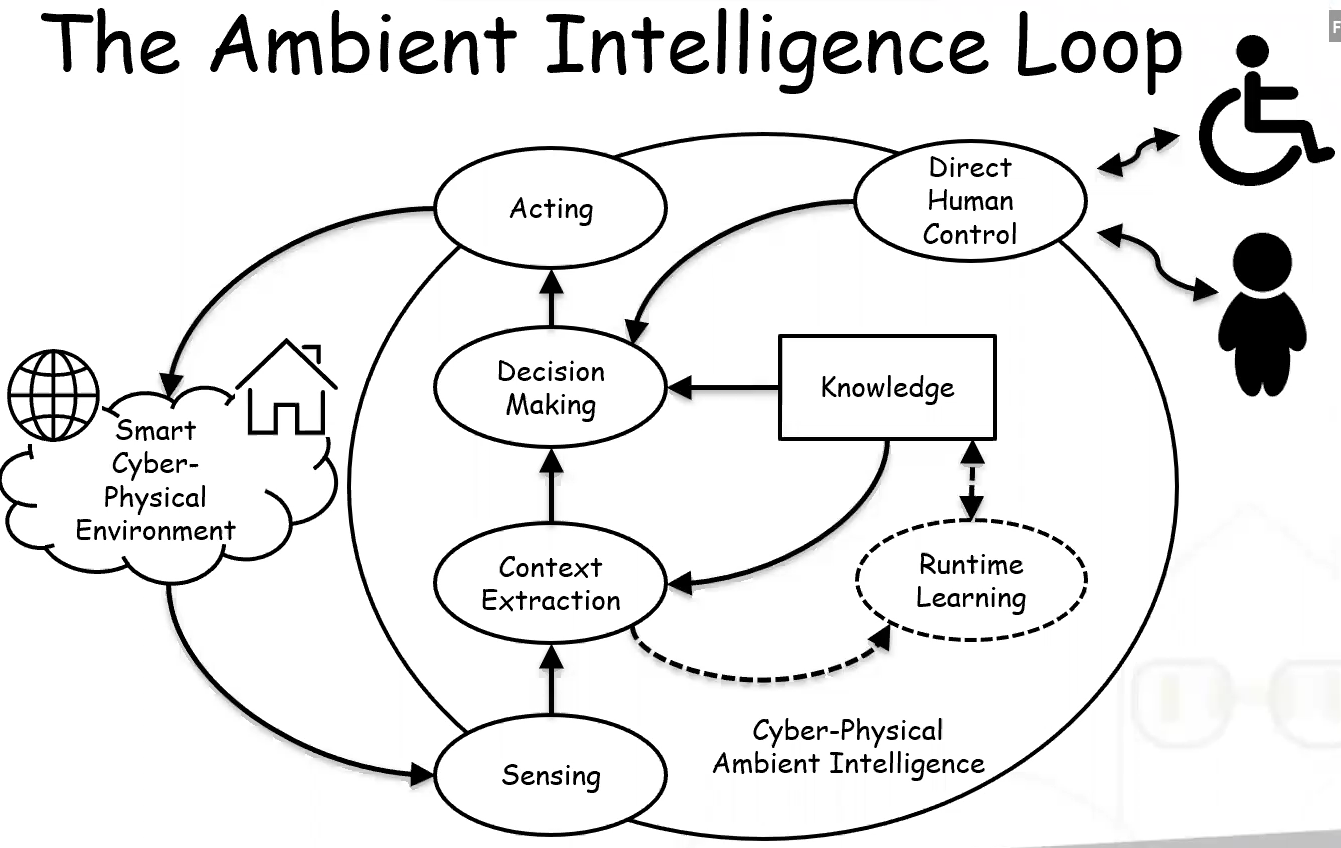
\includegraphics[scale=0.15]{./images/Ambient_intelligence_loop.png}
\end{center}

We have a smart cyber-physical environment (it's another concept often used to refer to a category that includes smart home), in which we have a set of sensors that sense the environment (i.e. they produce a stream of raw level data). With the data provided by the sensors we perform \textbf{context extraction}, which is a task that allow me to obtain a higher level of understanding of what is happening inside the environment. Once we did all our reasoning on the environment we can make some kind of decision on the environment. Next, we need to actuate such decision inside the environment, by using actuators that in turn change the environment. The step of context extraction and decision making are done accordingly to some kind of knowledge (manually defined or extracted by using some kind of machine learning method). We also have \textbf{runtime learning}, which is a component that refer to the need for adaptivity smart space. In addition we also have a \textbf{direct human control}, where the users will be involved in some kind of decisions. In particular, the knowledge component contains :

\begin{itemize}
\item \textbf{Context} : it's the state of the environment including the human inhabitants with their actions/activities/habits.

\item \textbf{Action} : it's an atomic interaction of the human with the environment or a part of it.

\item \textbf{Human preferences} : it's a specific set of rules over contextual variables. The goal here is the user satisfaction.

\item \textbf{Activity} : it's a sequence of actions or sensor measurements/events with a final goal.

\item \textbf{Habit} : it's a set of interleaving of activities that happen in specific contextual.
\end{itemize}

We can have different modeling methods such as :

\begin{itemize}
\item \textbf{Specification-based methods} : in this methods the knowledge is expressed in terms of some kind of logic language. Their major advantage is that they are usually human readable (if we are able to understand the language of the rules we are able to validate them). However, they are usually hand made by experts, and this is possible only with a feasible number number of sensors.

\item \textbf{Learning-based methods} : they are techniques taken from both machine learning and data mining (supervised, unsupervised and semi-supervised methods). Their main advantage is that they do not need any hand-made model. We need to underline that supervised methods still require a lot of labeled data. However, the disadvantage here is that they are usually not human readable, because they usually use statistical formalisms as HMM. In a smart space typically we use a supervised approach, which means that we have data coming from sensors, and we have the human that is in charge of labeling such data in order to let us learn some kind of model about human actions, habits, activities and preferences. Users usually do not like this kind of thing, because we are going to ask them for one week to label everything they do inside the environment. 
\end{itemize}

Each model has its own lifecycle constituted by the following components :

\begin{itemize}
\item \textbf{Specification/Learning} : it's the phase where the model is manually defined or learnt from data. The kind of learning techniques that we use has a huge impact on the following tasks, because according to the kind of things that we can understand during my context extraction phase we will be able to do specific things or not on my smart environment.

\item \textbf{Visual analysis} : it's the phase in which we analyze the model in order to understand if it's correct or not.

\item \textbf{Recognition and forecasting} : it's the phase in which we recognize that the model is actually valid in the current conditions of the environment. After the recognition phase, we can try to forecast what the user is going to do in the future.

\item \textbf{Anomaly detection} : it's the task for detecting if anything strange is happening wrt the model, and it's one of the first tasks performed in smart spaces.

\item \textbf{Decision making} : it's the task for making a decision on the environment, e.g. trigger an alarm, change the state of some actuator, etc.
\end{itemize}

We reported below a picture of a typical model lifecycle.

\begin{center}
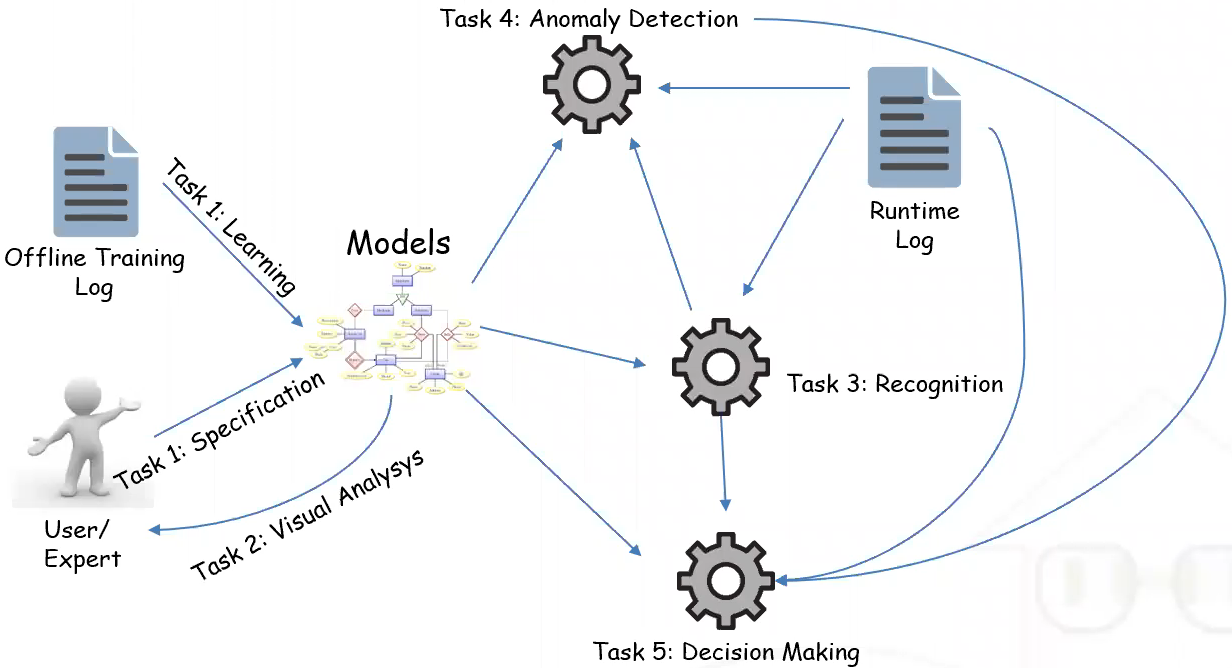
\includegraphics[scale=0.14]{./images/model_lifecycle.png}
\end{center}

In this picture there are two new concepts : \textbf{Offline training log} and \textbf{Runtime log}. The first one is a log consisting of raw level data acquired from the environment that has been labeled by the user or unlabeled if the system is unsupervised. Instead, the second one is a stream of data continuously coming inside the system and telling the system what the user is doing inside the environment or how the environment is evolving on its own. So, the offline training log is used in order to extract the model from the environment, while the runtime log is used as an input for the system in order to understand whether the user is performing some specific actions or he's deviating from the expected behavior.

\subsection{Specification-based methods}
The first logic approach in specification-based methods is based on Prolog, which is a logical based programming language mainly used in AI. In particular, we are interested in the "in-situation" operator, which captures a common form of reasoning in context-aware applications (i.e. it's used to ask whether an entity $E$ is in a given situation $S$). The advantage here is that reasoning about situations is completely decoupled from the acquisition procedure of sensor readings. Basically Prolog-based methods evolved over time into the Ontology-based methods. An ontology is a semantically rich conceptualization of a domain of interest, e.g. daily life and activities/habits. As in Prolog-based methods, the engineering effort is mainly in constructing the knowledge base, i.e. the ontology itself. Furthermore, ontologies are very difficult to be automatically learned. Most of the time ontologies are only used as a high level reasoning tool. In other cases ontologies are also used to assess the validity of the results obtained through machine learning methods. In addition to these kinds of logic, we have other logics such as LTL, Allen's Temporal Logic,  and Spatial Calculi.

\subsection{Learning-based methods}
In the vast majority of cases all the machine learning methods that are used in smart spaces are somewhat on the Bayes rule. The Bayes rule is a formula that tie the probability of a hypothesis $H$ giving an evidence $X$ as the ratio between the probability of $X$ giving $H$ times the probability of $H$ divided by the probability of $X$, i.e. $P(H \mid X) = \frac{P(X \mid H) \cdot P(H)}{P(X)}$. In the case of smart spaces, $H$ is our hypothesis (i.e. the user is performing a specific activity), and $X$ is the evidence (i.e. it's the output of the sensors or in general it's the input that we provide to the system). The problem here is that it's impractical to compute $P(X \mid H)$, and for this reason some relaxation over the Bayes rule are used in smart spaces. In particular, Bayes derivatives usually allows for learning and recognition. For example, a very basic method that is used in smart spaces is Naive Bayes (supervised method), which supposes variables in $X$ to be independent given $H$. We also have Bayesian network, which is basically a graph that tells us how different probabilistic variables influence one each other. An interesting version of Bayesian network is the Dynamic Bayesian Network (DBN) which introduce the notion of temporal evolution. One example are the Hidden Markov Models (HMM), which are DBNs where the system is assumed to be a Markov chain. A Markov chain is a chain of events where the next event is independent from the previous event given the current event. A HMM is constituted by a set of hidden states each with its own prior probability, the state transition probabilities and observation of the emission probabilities (the emission is basically what we are seeing inside the environment). The HMM main goal is to predict the current activity. Basically a HMM is built on three assumptions :

\begin{itemize}
\item Each state depends only on its immediate predecessor.
\item Each observation variable only depends on the current state.
\item Observations are independent each other.
\end{itemize}

An extension of HMMs are \textbf{conditional random fields}, where the probabilities of emissions and transitions are not constant, and the probabilities depend on the current subsequence of hidden states given previous emissions. Another technique frequently used in
smart spaces is \textbf{Decision Tree}, where we learn a set of decisions and we decide that we are in a certain activity given a set of decisions over the variables. \textbf{Support Vector Machines (SVMs)} is another technique frequently used in smart spaces. A SVM is a learning algorithm that allows us to obtain a separation hyperplane in a hyperspace. In the context of smart spaces, the hyperspace is a space where each coordinate inside the space is the value of the sensor. Then we look for the separation hyperplane in this space, that allows us to distinguish examples from one class to another class (the class is basically the activity that the user is performing). One of the main problem with SVM is that in the vast majority of cases the original hyperspace that we have do not allow for any separating hyperplane. So, what is done in SVMs is that this hyperspace is mapped to a very higher dimensional hyperspace using what is called kernel function. By default, SVMs are binary classification methods, but if we use $N$ different classification methods by having one class vs all the other classes, with the majority voting we can decide which is the most correct classification. Next, we have Artificial Neural Networks (ANNs), which is a network of neurons, where each neuron take a kind of signal as input, apply an activation function and output its signal to a following one. Basically we have a network constituted by different layers, where each layer is composed by specific types of neurons, and at the end it provides a kind of result. The problems with ANNs are that they typically requires a lot of training data and they are subject to the so called \textbf{curse of overfitting} problem (i.e. models do not generalize well). Actually the main goal ANNs are used for in smart spaces is basically to extract features for other learning methods. \textbf{Pattern mining} is a family of techniques that is used with sequence of events, and we try to extract patterns. These pattern mining techniques in the vast majority of cases are unsupervised techniques, but they integrate well with supervised techniques. The CASAS pattern mining approach is based on a compression mechanism : we try to map specific patterns to shorter symbols, and the more frequent is the pattern we are looking at the more short will be the symbol. Basically this approach works in the following way : it tries to always compress a little bit more the sequence of events, and in order to that it applies a kind of greedy algorithm to improve the compression that we have obtained. The compression is basically defined as the ratio between the description length of whole dataset, and the sum of the description length of the pattern that we have, and the description length of the dataset given the pattern, i.e. $Compression = \frac{DL(D)}{DL(P) + DL(D \mid P)}$. Let's look at other methods from the data mining research area that have been applied to smart space. When we talk about data mining the first algorithm that we can think of is the \textbf{Apriori algorithm}. It was invented in the $70$s and there the idea was the application to a supermarket. In a supermarket basically we want to know which kind of products are bought together by users, because if we know such association we may change the supermarket layout in order to place these products close one each other in order to help people to choose products but also to increase ourselves. In general, the goal of the Apriori algorithm is to find the set of frequent itemsets (we can think about itemsets as set of any kind). Basically when we apply this algorithm to AmI, we can use it in order to find sensors usually triggering together and sensors that when in specific state should trigger actions. An item is an assignment of a single variable to a single value out of its domain. An itemset is an assignment to a subset of these variables. In an itemset we cannot see the same variable more than once. The algorithm returns a set of frequent itemset. At a certain point an itemset can also be turned into rules. Instead, a transaction is an itemset that assigns values to all variables. In smart spaces transactions are equivalent to situations. A dataset in the smart space context is a sequence of transactions. The kind of association rules that the Apriori algorithm extracts are basically related to the most frequent itemset, i.e. given an itemset $C$, its support in $T$ is defined as $Supp(C) = \frac{T^{C}}{W}$, where $T^{C}$ is the number of times the itemset $C$ is in $T$ and $W$ is the total number of transactions and we say that an itemset is frequent if its support is above a minimum threshold value. Another technique for data mining that is frequently used in AmI is the \textbf{Emerging Patterns (EPs)} one. EPs are patterns of events that strongly characterize an activity or habit. An EP is an itemset that have a high support in $T1$ wrt its support in $T2$, where $T1$ is the set of transactions valid for a specific activity and $T2$ is the set of transactions from contrasting classes. In that case we are usually talking about supervised learning. Another approach that have been proposed is to automatically extract \textbf{event condition action (ECA)} rules for home automation. An ECA rule basically has the form "ON event IF condition THEN action", where condition can take into account time. ECA rules can be compared somewhat to decision making in AI agents (reflex agents). Let's see how these rules can be extracted through unsupervised learning. Basically we define three types of sensors :

\begin{itemize}
\item \textbf{Type O sensors} installed in objects, providing direct information about the actions of the users.

\item \textbf{Type C sensors} providing information about the environment.

\item \textbf{Type M sensors} providing information about the position of the user inside the house.
\end{itemize}

The events of the ECA rule always come from sets O and M, and the conditions are expressed in term of the values provided by Type C sensors. The actions part only contains Type O sensors called \textbf{mainSeT}. Then the algorithm proceed in the following way :

\begin{enumerate}
\item Discover for each sensors in the mainSeT, the set associatedSeT of O and M sensors potentially related to it as triggering events. We can use the Apriori algorithm to extract association rules that tells us that in a specific time frame a group of events are somewhat related between each other.

\item Discover the temporal relationship between the events is associatedSeT and those in mainSeT.

\item The conditions for the ECA rules are mined with a RIPPER learner (RIPPER is a seminal classification algorithm).
\end{enumerate}

Let's discuss the current limitations and opportunities that we have in the research community :

\begin{itemize}
\item We have seen that a lot of different algorithms, especially those that are fully based on supervised learning methods, require an extensive labeling, that is something that is feasible in the laboratory, but it's more difficult in real settings. In order to do that we can try to follow the Human in the loop approach (e.g. Nest thermostat). Alternatively we can use merge specification and learning based approaches, where the user tries for example to provide some basic rules, that could say what are the important actions that in the user opinion serves as a landmark for the beginning or the end of a specific activity. If we do not provide labeling, we provide at least segmentation. In segmentation, we have a dataset and basically we split it. Segmentation can be performed automatically using one of the following strategies : \textbf{explicit segmentation}, where the stream is segmented according to some kind of classifier, \textbf{time-based windowing}, which divides the entire sequence into equal size time intervals and \textbf{sensor event-based windowing}, which splits the entire sequence into bins containing an equal number of sensor events.

\item In several cases the recognition is performed, but it's coarse-grained. The recognition process just recognize which specific activity is ongoing, but it isn't able to help the user throughout the pipeline. In order to cope with this limitation there are some techniques that employs hierarchical models. 

\item The biggest problem about the application of AmI techniques to smart space in real scenarios, is the problem of multiple users. When we are in a smart house, it's very difficult for the smart house to understand whether a specific activity is performed by human $A$ or human $B$, because in the vast majority of cases we don't have any tracking and localization system in the smart house. One way for example to understand which specific human perform a specific activity is to equip all the devices and sensors that we have in the house with tags.

\item Another big problem is the problem of knowledge update.

\item Another limitation is that many of these learning based method are not easy to be validated by the end users, and this holds especially for supervised learning based method.

\item Also the visual analysis is a big problem.
\end{itemize}

When we try to create our own algorithm in smart spaces we must to face the problem of which dataset we use to validate it. We can decide to equip our own smart house and to acquire the data, but acquiring the data, especially labeled one, is expensive. There exists several alternatives such as datasets provided by CASAS project. However these datasets do not have a standard format, and we don't have any guarantee about the quality of labeling since the labeling is done by humans. Also another limitation of such datasets, is that they contains a very limited number of sensors. An interesting feature of WSU datasets is that they also provide the smart home in a box kit, which is freely distributed by WSU to research groups, and allows to perform simulation and crowdsourcing. Another interesting dataset is provided by Tracebase, which contains power consumption traces collected from individual electrical appliances.

\subsection{Habit mining}
Let's start where the idea of habit mining come from. Habit mining is a technique to extract human habits from logs. We start by introducing the concept of \textbf{business processes}. A business process is a set of activities that are performed in coordination in an organizational and technical environment to realize together a business goal. A business goal is the target that an organization aims to achieve by performing correctly the related business process. Actually business processes are at the core of most information systems such as the production line of a car manufacturer. In order to create this information system the customer specify its business processes for the orchestration of participants, information and technology for the realization of products and services. An information system that supports a business process is called \textbf{Process Management System (PMS)}. The PMS takes as input a model of the process, and it routes the different tasks to the different resources. A PMS is driven by a specific business process model. There are actually different ways to classify business processes :

\begin{itemize}
\item \textbf{Structured} : in this case we have processes that are completely predictable.

\item \textbf{Structured with ad hoc exceptions} : this kind of processes are very similar to simply structured processes, but in this case we also have an explicit description on how we should face exceptions.

\item \textbf{Unstructured with pre-defined fragments} : in this class of processes the process modeling could not be completed before the execution.

\item \textbf{Unstructured} : in this case it's impossible to define a priori the exact steps to be taken in order to complete an assignment.
\end{itemize}


Process mining emerged in the $1998$ in the software engineering field with Cook and Wolf. Process mining was initially described as the ability to discover process models from event-based data. The process mining main goal is to seek the confrontation between event logs (i.e. observed behavior) and process models (i.e. expected behavior). We reported below the usual workflow of process mining.

\begin{center}
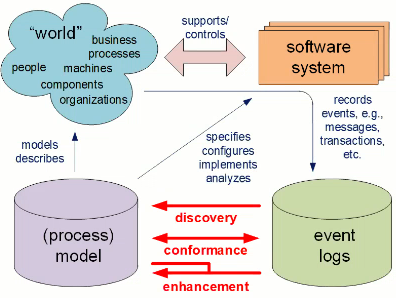
\includegraphics[scale=0.5]{./images/process_mining_workflow.png}
\end{center}


In particular, process mining is constituted by the following components :

\begin{itemize}
\item let's start from the world. We have a world which is made up of people, machines, organizations, computer systems and business processes. In order to control this world we use software system (PMS).

\item This software system have logs, it record what happens because it is helpful in order to recover from crashes, but also for responsibility issues. These logs are usually not very well structured and we can integrate them in order to obtain event logs.

\item At this point we can \textbf{discover} a process model. Discover means extracting from the event log the graphical representation or the rules that are behind the processes. Next, we can perform \textbf{conformance}, with which we compare process models with event logs. Then we have \textbf{enhancement}, with which we take more recent event logs in order to enhance our process models in certain cases.
\end{itemize}

All the previous process mining techniques are actually easily available through a set of commercial or open-source tools such as ProM, Apromore, Disco, etc. The structure of an event log in a business process (which concern a single process) is constituted by different cases. A case is a single execution of a process. Then inside each process we have a sequence of events for which we have an event id, a timestamp, the specific name of the action and other features. Another thing we must be aware of is that activities in process mining have a different meaning wrt smart spaces, because activities in process mining corresponds to actions in smart spaces. Instead processes in business processes corresponds to activities and habits in smart spaces. In order to describe the event logs in business processes we have a standard called \textbf{eXtensible Event Stream (XES)}. It's basically the evolution of XML. The idea that we have to apply BPM and processing mining to smart spaces is the following : we have raw level of information where we have sensors and actuators and we have the higher level where we have processes. Then we have to merge these two visions of the world by using event processing and learning, which correspond to the context extraction feature discussed in AmI. Of course BPM allows to describe the high level of knowledge, whereas IoT works at the low level of knowledge. The advantage of using process mining is that we have great benefits from the point of view of visual analysis, because processing mining actually wants to produce process models, and this latter are intended to be easily readable from the end users. Process mining is ground in logs and very descriptive, and they are a kind of trade-off between specification-based and learning-based methods. The first challenge to be addressed is the problem of granularity between the granularity of sensor logs and the traces used for process mining. In other words, we cannot find a one-to-one correspondence between sensor measurements and performed actions, because a single user action may trigger many sensor measurements, and a single sensor measurement may be related to several actions. So, the first step to apply process mining to smart spaces is to aggregate sensor measurements to recognize actions. Next, we can apply process mining. A prerequisite that we have in process mining is that an event log must be explicitly segmented into cases and we need to explicitly define when a case "start" and when a case "end" and for each event which case it belongs to. We need to define correspondence between processes and human activities, manage the problem of multiple users, and which formalism we intend to use. However, human processes in smart spaces are very similar to "artful" processes (e.g. treating patients in hospitals), and this means that the resulting graphical representation of BPM is unreadable. Our approach to apply BPM to AmI is called \textbf{visual process maps}, which is based on fuzzy mining. Fuzzy mining is a particular type of BPM, where we treat a process as it's basically a geographical map. So, we start from a smart environment, we acquired the sensor logs, visually analyzed the content of the log and extracted model of human habits. The dataset that we used is the Aruba dataset from CASAS project, which contains information about the life of a woman for two years. The input to our tool besides the data file containing the dataset includes also a map of the house and file which contains information about the position of each sensor in the house. One of the problem that we have is that we must segment the data. In particular, we decided to perform a very simple segmentation. We imagined to obtain a process model of the daily habit of the person, i.e. we want to obtain as single model that describe all the entire day of a person looking at the dataset. The first tool that we have in the log, is the player because it tries to play the dataset inside the environment. We can choose which sensors include in the house, select the simulation speed, etc. At the end what this tool does is as soon as we click on play, we will see animating the path that is followed by the person on the map by looking at the sensors. At each step we have a dot which reflects the time spent under each sensor in the path. At this point, we can compute subtrajectories in order to turn sensor measurements into actions. In order to accomplish this task we applied the TRACLUS algorithm (it's a seminal algorithm), which takes a sequence of sensor measurements and returns a set of segments. At this point, we used a simple classification technique based on a linear combination of factors in order to classify each of these segments in movement action : STAY (stay at a specific place), AREA (moving inside an area), MOVEMENT (moving from one area to another area of the house). In order to perform this classification we computed for each segment the following indicators : $I_{m}(\delta)$ reflects how many sensors are involved in the trajectory, i.e. $I_{m}(\delta) = \frac{\# distinct \hspace{0.1cm} sensors}{\# sensors}$, $I_{a}(\delta)$ reflects how trajectory time is distributed among sensors (Gini coefficient) and $I_{s}(\delta)$ reflects how much time is spent under a single sensor, i.e. $I_{s}(\delta) = \frac{time \hspace{0.1cm} spent \hspace{0.1cm} under \hspace{0.1cm} the \hspace{0.1cm} most \hspace{0.1cm} frequent \hspace{0.1cm} sensor}{total \hspace{0.1cm} time \hspace{0.1cm} of \hspace{0.1cm} trajectory}$. At this point in order to classify each segment provided by the TRACLUS algorithm, we defined the following thresholds :

\begin{center}
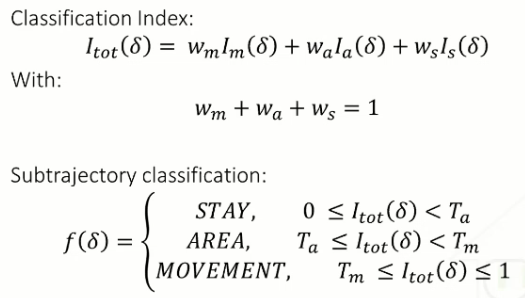
\includegraphics[scale=0.5]{./images/BPM_thresholds.png}
\end{center}

So, given the original dataset, we transform it into a sequence of subtrajectories, where each trajectory is a specific action. Next, we apply fuzzy mining, using as segmentation the entire day (in this case we used only STAY and AREA actions). Now, we moved to a more complex setting, where instead of describing the entire day of a person we tried to extract real habits. In order to do that we treated time dimension as a continuous attribute to be discretized (e.g. by applying chi-merge) and we tried to experiment a little bit with inductive miner instead of fuzzy miner. Basically, we started from the coarse-grained dataset and segmented it in units of $15$ minutes. Then at each iteration we applied process discovery to each segment, we computed the quality measure of the process called \textbf{structured and simplicity}, we find the best pair of adjacent intervals according to these metrics, and then we merge adjacent time zones and we stop when we reach the best description of the day in term of process model. Producing the heat map we were able to associate each activity with temporal intervals in which the activity occurs more frequently. Next, we have to associate each habit with the activities that occur more frequently in that temporal interval.

\subsection{Smart manufacturing}
Smart manufacturing also known as industry $4.0$ is the evolution of the traditional world of industrial automation, thanks to the continuously evolving technologies for networking, storage and computing. The smart manufacturing main goals are to increase the productivity and quality, ease workers lives and define new business opportunities. A Digital factory is a key concept of industry $4.0$, which is defined as a multi-layer integration of the information related to activities along the factory and related resources. The emerging trends connected to industry $4.0$ are that factories and machines are increasingly complex (human-centricity and robot collaboration are crucial), mass customization (customers requires customized services and products), business processes are not considered isolated anymore and smart supply chains (it's defined around the concept of agility, a mix of responsiveness and adaptivity, and dynamic situations, that must be managed during the product lifecycle).  In order to define in details what is smart manufacturing, a german initiative introduced the \textbf{Reference Architectural Model for Industry 4.0 (RAMI)} definition. RAMI is constituted by three components :

\begin{itemize}
\item \textbf{Life cycle value stream} : it tells us that in order to talk about smart manufacturing we must follow the entire value stream of the product, that goes from the design and development of the product, to its production and maintenance.

\item \textbf{Hierarchy level} : it tells us that all the phases in the product life cycle must be imagined from the point of view of the different facilities that cover different aspects of the single phases.

\item \textbf{Logical layers} : we look at all of these combination of the life cycle phases and organizational level, from the point of view of :

\begin{itemize}
\item \textbf{Asset layer} : they are physical components such as robots, but also non-physical objects such as software and ideas.

\item \textbf{Integration layer} : it takes the information from the assets in a form that can be digitally processed (i.e. Digital Twins).

\item \textbf{Communication layer} : it's the standardization of communication using uniform data format and predefined protocols.

\item \textbf{Information layer} : it process and integrate available data into useful information.

\item \textbf{Function layer} : it includes the formal description of functions.

\item \textbf{Business layer} : it includes the mapping of the business model and links between different business processes.
\end{itemize}
\end{itemize}

A \textbf{Digital Twin (DT)} is a digital representation of a physical thing. This means that basically DTs can come in many different forms in digital factories processes such as humans and industrial machines. DTs are a faithful representation in the digital world of a physical entity. DTs usually provides a software interface (APIs) to receive instructions and to query data, connectivity, autonomy, homogeneity, customizability and traceability. If we have a DT we can describe it from the point of view of service interfaces that it provides :

\begin{itemize}
\item \textbf{Sync} : they are interfaces that are made up by synchronous methods, i.e. we issue a command and we wait for the command to be completed.

\item \textbf{Query} : they are interfaces that allows to query DT data.

\item \textbf{Async} : they produces asynchronous data describing DT activity and status.

\item \textbf{Simulation} : this kind of interfaces performs predictive monitoring.
\end{itemize}

Of course for each DT interface we can have a more or less formal specification. The most known frameworks to implement DTs are Ditto, Bosch IoT Things, Azure Digital Twins and AWS IoT Device Shadow. In industry $4.0$ it's fundamental to understand how the data space of a digital factory is organized. In particular, we can have the classical systems, but also machines and information systems that are complex and heterogeneous (different vendors, standards and vocabularies). Furthermore, in many cases data are not available in the form of databases, and the information that we can obtain from the DT is limited to the one that we can obtain from the services that describe the DT that wrap it with the machine. Additionally we don't have an interaction with DTs that is only synchronous, because we can have an asynchronous interfaces for example when we have huge data volumes coming from sensors. In addition, we don't only have data about the current situation of the machine, we also have information the past situations of the machine, and thanks to the prediction feature we also have information about the future of the machine. In the data space, we have to consider that we don't only have information from our own factory, but we also have information from other factories that belongs to the supply chain. Simulation is something that allows us to predict what is going to happen to the physical entity between the DT and this concept is built around the concept of \textbf{Experimentable Digital Twins (EDTs)}. EDTs provides us a set of functionalities that allows us for example to obtain the so called remaining useful life of the machine, i.e. how much time our machine will last ? In predictive maintenance is constituted by different levels :

\begin{itemize}
\item \textbf{Level 1 : Reactive} : we don't really have a plan, whenever something got broken we asks somebody to fix it or we fix it.

\item \textbf{Level 2 : Planned} : we know that certain machines must be periodically checked, and we have a plan for this.

\item \textbf{Level 3 : Proactive} : we proactively act on the machine in order to improve performance. For example we fix a machine before it got broken.

\item \textbf{Level 4 : Predictive} : it's based on advanced analytics and sensors that tells us when the machine will broke. (e.g. die cutter project).
\end{itemize}

\subsection{Automated synthesis in smart manufacturing}
In a factory we need a compositor that is able to synthesize a plan for the factory as soon as a human supervisor produces a production goal. How can we implement this compositor component ? Usually AI manages this control problem (select the action to do next) using three approaches :

\begin{itemize}
\item \textbf{Programming-based} : specify control by hand. The domain-knowledge is easy to express by creating rules, but we cannot deal with situations not anticipated by the programmer.

\item \textbf{Learning-based} : learn control from experience. We can use an unsupervised (reinforcement learning), supervised or evolutionary approach. The advantage of these approaches is that they do not require much knowledge in principle. However, in practice we  require to work on the right features.

\item \textbf{Model-based} : we specify the problem by hand, and derive control automatically using Automated Planning. A DT could be modeled as a guarded automaton by extending the work from the early 2000's papers on service composition. There are differences between web service guarded automata and DTs ones : the local storage contains not only data from caller and instantiated by the automata, but we have data also coming from sensors and predictive monitoring and data from other DTs, and we have two different perspective, the actual one is for the real-world data, while the simulation one is for the simulation world data. In web service composition, a target service is the goal of the composition where the compositor is based on an unique data schema, the target service is described as an automaton itself and the set of available services is known a priori and cannot change. In DTs composition a target goal or KPI must be defined in a declarative manner and no unique data schema is available, and the compositor must be able to discover new DTs at runtime. Another possible approach is the one based on automated planning, where the (classical) planning is to find a sequence of actions that  transforms an initial state into a goal state (this is called a plan). States are truth assignments, represented by the atoms that are true. The actions add certain atoms and delete others, provided their preconditions hold. A planner is a solver that takes as input a planning problem and a planning domain and outputs a plan. The cost of a plan is given by the sum of action costs (default is 1). In order to specify the planning domain we can use several definition languages such as \textbf{Planning Domain Definition Language (PDDL)}. 
\end{itemize}

Now let's look at an example of employment of planning in the case of smart manufacturing. We have a manual description of the process that goes on in a smart factory. At each step we have different products that follow different steps in the chain, and some of these steps can process different items at once. If something wrong happens, we must find a solution in order to allow the process to continue. In BPM we can have either \textbf{anticipated exceptions}, which are things that we expect (so we provide a strategy in order to face these kind of problems) or \textbf{unanticipated exceptions}, which are exception that we cannot imagine when we define the process. We can imagine to model our ideal process of our factory as basically using a situation-based approach. Now, instead relying on the fact that the process will go always well, after the execution of each step we have two different reality : we have the \textbf{expected reality}, which is the reality we expect after the execution of the action in a specific situation, and the \textbf{physical reality}. If the expected reality is equal to the physical reality that we obtain after the execution of a task then the process is going well. Otherwise, we must fix the process via planning, which tells us how to modify the physical reality in order to obtain the expected reality. Once we have the expected reality we can continue with the usual process. This is automatically done by planning and it's called \textbf{SmartPM}. Recently we stack thinking to the different ways to apply planning in smart manufacturing. We defined a system called \textbf{AgiLe Twin Orchestrator (ALTO)}, which takes as input the description of DTs in the context of the DT framework, we take a production goal and we automatically orchestrate the different DTs by using the DT framework in order to reach this goal. We defined the entire process as soon as something wrong happen we're also able to decide whether to fix the process for the specific item or to switch to mass production. The limitations of this approach are the following : the preconditions and effects of DT actions are expressed as conjunctions of boolean predicates, different DTs share a common vocabulary, and planning takes into account neither non-determinism nor probabilities in the execution of DT actions, thus resulting potentially non-optimal or risky plans. 


\section{Robotic process automation and process mining}
Robotic process automation (RPA) is a fast-emerging automation technology, based on the notion of software robots that allows organizations to automate high volume routines. SW robots are mainly used for automating repetitive office tasks in operations like accounting, billing and customer service. SW robots are capable of emulating the actions of a human worker such as log into applications and connect to system APIs, copy and paste data, etc. So, a SW robots is usually developed to capture the execution of the tasks previously performed by a human user on the UI of a computer system, and then to emulate the automation of such tasks in place of the user. RPA evolved from three key technologies :
\begin{itemize}
\item \textbf{Chatbots} : they are software applications that helps an user to perform an activity on a website.

\item \textbf{Screen scraping} : it can be considered a kind of data mining technique that is able to understand what is happening on the screen of a computer system and they're able to derive the information that are flowing inside this screen, and show such information via modern user interfaces.

\item \textbf{Workflow automation} : it refers to all those techniques that allow to design and executing automation of processes based on workflow rules where human tasks, data or files are routed between people or systems based on pre-defined business rules.
\end{itemize}

Now, how a RPA project is conducted ? To do that we need the following steps :
\begin{enumerate}
\item We need to determine which routines are good candidates to be automated. This requires the support of skilled experts that identify the candidates routines to automate by means of interviews.

\item Model the selected routines in the form of flowchart diagrams that define the behavior of a SW robot.

\item We taking any flow chart and generate the SW code required to enact the associated SW robot on a target computer. The issue here is that often there is a misalignment between 1) and 3), the designer adjust the flowchart diagram to fix the identified gap, in order that the robot's current behavior matches the robot's expected behavior. It's a trial-and-error procedure until success.

\item Deploy the SW robots in their environment to perform their actions.

\item Finally, we maintain the routines over time to eventually enhance their behavior.
\end{enumerate}

Now, how can we inject more automation inside steps 1)-2)-3) ? An idea could be to use process mining techniques. So, process mining is a group of techniques that is able to compare event data (i.e. observed behavior)  against process model (expected behavior). Any execution of a process model produces a new execution trace recorded in an event log. An event log consists of several events, where each event corresponds to a particular activity execution. There are three main process mining techniques : \textbf{discovery}, \textbf{conformance} and \textbf{enhancement} (see Smart environment seminar). Process discovery is about to have an event log as input, analyze it and build the corresponding process model. About conformance checking, is to take as input an event log and a process model to find out discrepancies. Typically, we use the replay technique with which we replay the traces of a given event log on top of a given process model. Now, the idea is to use these techniques in order to inject more automation into the current RPA technology, towards a new methodology to conduct a RPA project :

\begin{enumerate}
\item First of all, we record the mouse/key events that happens on the UI of the SW applications involved in a routine execution (UI logs).
\item Automatically determine which routines are good candidates to be automated by analyzing the UI logs.
\item Automatically model the selected routines in the form of flowchart diagrams that define the behavior of a SW robot interpreting the UI logs.
\item Develop each modeled routine by automatically generating from UI logs the SW code required to enact the associated SW robot on a target computer system.
\end{enumerate}

Nowadays there exist 55 providers offering RPA solutions with different prices and functionalities. Intra-routine self learning means that the RPA tools are not able to associate automatically user actions to executed routines. UI logs are characterized by long sequences of actions that reflect a number of routine executions. Indeed, a log can record information about several routines, whose actions are mixed in some order that reflects the particular order of their execution by the user. The challenge is to automatically understand which user actions contribute to which routines inside an UI log. This is issue is known as \textbf{segmentation}. The second issue is called \textbf{intra-routine self learning}. It's often performed by means of interview, direct observation of workers. The third challenge is to automatically generate flowcharts and synthesis of SW robots (this requires high quality UI logs). Starting from these challenges we can derive  the \textbf{SmartRPA methodology}, which consist of recording the activities performed by an user, and then exploit conformance checking to identify which activities belongs to which routine. So, the idea is that we can perform the segmentation task. The routine traces can be stored in different routine-based logs, and we can apply to them process discovery technique to derive the flowchart of the routine itself, and we can finally generate the SW code for the SW robot to correctly emulated the target routine.\\\\Now, let's analyze a supervised approach to segmentation. The scenario concerns the filling of a Google Form using the data from an Excel spreadsheet containing the information to apply for a travel request (Routine 1). In addition, if the request applicant declares that s/he would like to use her/his car as one of the means of transport for the travel, then s/he has to fill a dedicated web form (Routine 2). There are many different variants of UI logs that can be analyzed :

\begin{itemize}
\item \textbf{case 1} : the UI log include just one single routine, and the routines are executed one after the other.

\item \textbf{case 2} : the routines interleaves between each others.

\item \textbf{case 3} : we can have many routines executions that can be interleaved.
\end{itemize} 

Analyzing the existing techniques, we discovered that they are able to perform segmentation in the simplest cases 1.1. and 2.1. The idea is to use \textbf{trace alignment}, which investigate relations between moves in the log and moves in the model to establish an alignment between a given model and a trace. The outcome of such technique is a number called \textbf{fitness}, which quantifies how much the trace deviates by the model. 


\section{Modern approaches to entity resolution}
Data integration is about discovering knowledge about real world entities. An entity in the real-world can be anything like a person, book, place, etc. We discover knowledge by combining data from a variety of sources and we want to provide users with an unified view, so that users can go through those data artifacts in details and possibly discover more information. This is something that people and companies like to do because it's either their core business or as a building round for more advanced applications. For data integration we have a pipeline of tasks to follow : first of all we have data extraction (i.e. collecting data from a source), schema alignment (i.e. resolve columns), entity resolution (i.e. resolve rows), data fusion in order to discover conflicting values and identifies which values are correct and eventually we can build advanced data artifacts (i.e. we can build the so called knowledge graphs). The main types of ER problems are the following :
\begin{itemize}
\item \textbf{Structured ER} : it's a variation of ER that takes as input structured records and we imagine that we already solved the schema alignment.

\item \textbf{Semi-structured ER (variant 1)} : in this case we have structure records, but the schema alignment is not perfect.

\item \textbf{Semi-structured ER (variant 2)} : in this case the schema alignment is correct, but some attribute values may appear under the wrong attribute.

\item \textbf{Textual ER} : in this case we don't even have attributes, we have just long descriptive strings and we want to understand which descriptions refers to the same real-world entity.

\item \textbf{Unstructured ER} : in this case the input are images and multimedia.
\end{itemize}

Solve an entity resolution problem means that we get a set of records from multiple sources, and given two records we say that they matches when they refers to the same real-world entity. The ground truth of this problem is a complete labeled graph having two types of edges, positive and negative edges, and this solution is a clustering that is transitively closed. In other words, it means to partition the graph into cliques, where each clique represent a real-world entity. In particular, we take as input a set of records, and the first step is to reduce the search space for duplicates, i.e. it means that we want to exclude trivial non-matches. Next we need to recognize duplicates, i.e. for every pair we have to decide whether my guess for the edge is positive or negative, and finally we need to do clustering, where we need to decide whenever there are edges that conflict with the transitive property of the ER problem, and we have to decide how to color the edges whether green or red. Now, suppose that we want to evaluate a pipeline implementing this paradigm and solving ER. In this case we have two goals : we want to be both efficient and accurate (we don't want only to be fast, but we want to return also a correct solution). Accuracy is a complex objective because it can be defined under multiple perspective such as precision, recall, F-measure and an advanced measure called progressive F-measure. In particular, we can use the first three measures for evaluating the duplicate elimination task. In we want to evaluate the entire pipeline, we have other things to take into account. So, the cost is proportional to the number of queries to the duplicate recognition tool and we user the progressive F-measure, where we plot the F-measure as we go and we consider the area under the F-measure against the cost curve. Of course we want to maximize progressive F-measure, but it depends on the order of queries to the duplicate recognition tool. Find the right order is hard, but we can use prior matching probabilities computed those based on functions like string similarity and see which one is more promising. If we are willing to solve this task by maximizing progressive F-measure, the first thing that we need to be able to compute is string similarity, because it's able to guide us for example in the ordering of the queries. String similarity is just a measure of how close two words or sentences are (close is terms of letters). Another issue that is useful to solve if we want to compute ahead the similarity of things because we want to maximize for instance progressive F-measure, is that we want to care about syntactic similarity and also to care about semantic similarity. Let's see how we can optimize the F-measure. For computing the similarity between strings there is a variety of algorithms which are divided in two categories : 
\begin{itemize}
\item \textbf{Edit based metrics} : they measure how many characters needs to be changed in order to make two strings the same. An example of this type of metric is Soundex, which has the intuition of encoding words close if they sound the same in english. It consists of the first letter of the name followed by three numbers, where numbers encode similar sounding consonants. Another metric is the edit distance algorithm which truly computes the operations that are needed to transform one string into another, and the edit distance is measured as the length of the shortest sequence of operations to transform one string into the other. However this method is expensive because is quadratic on string length in the worst case. Another algorithm is called Jaro, which aims at measuring the difference in terms of characters, but it's more complex than the edit distance algorithm. The intuition is that we want to compute how many transpositions we need to convert one string into the other.

\item{Term based metrics} : they are more focused on tokens. An example of this kind of algorithm is Jaccard, where we just take two sets of terms S and T, and we can compute the Jaccard coefficient as the fraction between the size of the intersection between S and T, and the size of the union between S and T. Another approach is to use the tf-idf value, where tf denotes the number of times term appears in a document, and idf denotes the number of documents containing that term. Such value is defined as $\log (tf + 1) \cdot \log (idf)$. Another way to measure the similarity of two strings based on terms is the cosine similarity. In this case we can transform a set of terms into a sparse vector S of high dimensionality, weighting it via tf-idf or tf score.
\end{itemize}

The previous algorithms are in charge for discovering syntactic similarities between two words, while a good way for representing semantic similarities of terms is to look at their context. In order to take context into account, we can build a model that predicts the context by giving as input a word (e.g. Word2Vec system). Typically we make a massive usage of pre-trained systems give us embeddings and compute their cosine similarity. Now, how do we use all those things to really decide ? The literature provides several methods that are all based on four main steps :

\begin{itemize}
\item \textbf{Step 1} : we use word-embedding to represent tokens or terms in the dataset.

\item \textbf{Step 2} : we reuse well known techniques for nlp processing to summarize and compare attribute values.

\item \textbf{Step 3} : we use a classification system to decide those vectors representing not its related terms, but representing entire records whereas match or not match.

\item \textbf{Step 4} : we use string similarity to generate non-trivial negative examples for training.
\end{itemize}

\subsection{Modern approaches for clustering and reducing the duplicates search space}
In this context we want to build clustering system with high progressive F-measure. Let's first ask ourselves what is the minimum number of queries that we need to ask in order to declare that our solution is complete. At a first glance, we might be tempted to say that the number of queries to the oracle that are needed is something like quadratic. This is not really true, because in many settings that number can be much less thanks to transitivity. So say that we have in the ground truth $K$ clusters and we have $N$ records that we need to partition. If we have an accurate duplicate recognition tool the number of queries that we need to ask for completing my task is $N - K + {K \choose 2}$, because for discovering one cluster of size $c$ the number of queries that we need is precisely $c - 1$ and we need additional ${K \choose 2}$ queries because for every pair of clusters we need only one query with a negative response. We predict the ordering of the queries by estimating the matching probability, next we calibrate these probabilities using a sublinear sample of pairs. Then we will forget how do we decide whether two pairs are matching or not, because we will treat the whole duplicate recognition step as a black box oracle, which has one property that is the fraction of erroneous answers. The easiest strategy for ordering the queries is by ordering the edges by decreasing probabilities. This strategy is good but it's has quite high approximation ratio. The second strategy orders nodes in order of their expected cluster size (i.e. the sum of probabilities of incident edges). This strategy is better than the previous one, because the approximation ratio is linear in the number of clusters and not in the number of nodes. A third strategy called \textbf{Hybrid ordering} not only promotes matching edges in expectation with high probability and promotes larger clusters with high expected size, but it also include a method for sticking for one cluster when it started growing that. Now, what if in this entire framework some edges are erroneous ? So we can implement and deploy an error correction layer such that when my strategy will instruct me to query one specific edge because from the optimal ordering perspective is the most promising one, my error correction layer will kick in and not just query that edge, but query a random subset of control edges in order to validate the answer of the duplicate recognition tool.\\\\Reducing the duplicates search space is a slightly different than the one that we have been discussed so far, and in a sense requires a new problem statement. We have as input a set of records, we don't want to return partitions (this is the goal of the entire ER step), we want just to return a subset of pairs possibly not even transitively closed consisting of the most promising pairs for further consideration in the remaining steps about duplicate recognition and clustering. There is one way to do that that is called \textbf{blocking}. So, given a set of records, we will group records into blocks that are possibly overlapping, and then we will return as output a subset of edges that connects nodes sharing the same block. So, here we don't care about precision, we only care about recall. So by considering this problem statement, we can though to the process solving it again as consisting of three steps : \textbf{Block building} in order to partitions all the records in blocks, \textbf{Block cleaning} in order to remove unwanted blocks, and \textbf{Comparison cleaning} in order to filter out some edges to get one nicely sparse graph that can be submitted as input to the duplicate recognition and clustering steps. One way for building blocks is called \textbf{standard blocking}, creates a block for each token and then maps records into blocks by simply asking if that token is included in that record. Another way to build blocks is to use the \textbf{approximate nearest neighbors} approach, which build a clustering of the nodes for example via LSH and then blocks are somehow circles or hyper spheres in the embedding space. To decide which blocks are too big we case use TF-IDF of the corresponding term (it promotes small blocks), or we can use the entropy which promotes clean blocks (i.e. more uniform). Comparison cleaning can be done for instance by meta blocking. It means that we take as input the blocking graph (i.e. a graph where there is one edge if two nodes shares at least one of the remaining blocks) and we need to make it sparse. In this graph each edge is weighted by using block scores and then we prune in two main schemes : either we keep the top $K$ edges incident on each node or we keep the top $M$ edges overall. One method for block building is based on deep learning, where for each word we can build an embedding, we can then represent a summary of all the word embeddings of a tuple regardless of its schema, and then we can submit to the similarity layer not the pairwise attribute-value representation, but we can just submit directly the pair of the vector representation of the two tuples, and learn similarities.

\subsection{Explainable AI methods for entity resolution}
It's true that AI methods provides us more accurate approaches for entity resolution, but they make them more opaque. In other words, we don't want only accuracy approaches for ER, but we want also that they are interpretable. There is a plethora of methods for making AI methods interpretable. The first partition is \textbf{features-based vs samples-based}, where in the first method the explanation is based on the features in the data, while in samples-based a target class has been learned such because of specific samples in the training data. The next partition is \textbf{local vs global}, where local methods aims at describing the behavior of a single prediction, whereas global aims at describing the behavior of the entire model. Then we have \textbf{static vs interactive}, where static methods provides explanations without asking any feedback, whereas in interactive methods we have nice graphical interfaces, and the users can interact with the explanation system. Another approach is \textbf{directly interpretable vs post-hoc}, where directly interpretable means that we're changing the model by making it more transparent, while post-hoc means that the explanation system involves an auxiliary method that aims at explaining a model already in place and trained that we do not change. We can do that by building a \textbf{surrogate model}, which is a model that is much more simpler, interpretable and that resembles and approximates very well the original complex and opaque model, or we can just build \textbf{visualizations} of intermediate layers for instance if we have a neural network, to give people more intuition of the inner working of the model. Finally the last categorization is \textbf{black box vs white box}, where black-box methods do not need to know the inner properties of the method, because they're based on perturbation of the data and see how the model reacts to perturbation. Whereas white-box methods rely on the internal mechanisms of the model. 

\end{document}